% ========================
% estilo.latex mínimo funcional
% ========================

\documentclass[12pt]{book} % report para capítulos

% ========================
% Paquetes y comandos extra
% ========================
% ===========================
% Paquetes básicos de idioma y codificación
% ===========================
\usepackage[utf8]{inputenc}   % Codificación UTF-8
\usepackage[T1]{fontenc}      % Acentos y caracteres correctos
\usepackage[spanish]{babel}   % Traducción al español (capítulos, índices, etc.)
\usepackage{csquotes}         % Citas tipográficas correctas

% ===========================
% Tipografía
% ===========================
\usepackage{lmodern}          % Fuente Latin Modern
\usepackage{microtype}        % Mejoras tipográficas (espaciado, justificación)

% ===========================
% Márgenes y geometría
% ===========================
\usepackage{geometry}         % Control de márgenes
\geometry{a4paper, top=3cm, bottom=3cm, left=3cm, right=3cm}

% ===========================
% Matemáticas
% ===========================
\usepackage{amsmath, amssymb, amsthm} % Paquetes AMS
\usepackage{mathtools}        % Extiende amsmath
\usepackage{physics}          % Notación física y matemática (derivadas, bra-ket, etc.)
\usepackage{siunitx}          % Unidades SI (e.g. \SI{3}{m/s})
% \sisetup{locale=ES}           % Configuración para español (coma decimal, etc.)
\AtBeginDocument{\RenewCommandCopy\qty\SI} % Resolve siunitx and physics conflict


% ===========================
% Gráficos, tablas y colores
% ===========================
\usepackage{graphicx}         % Insertar imágenes
\usepackage{xcolor}           % Colores personalizados
\usepackage{tikz}             % Dibujos vectoriales
\usetikzlibrary{calc,positioning,shapes,arrows} % Librerías útiles de TikZ
\usepackage{pgfplots}         % Gráficas de funciones
\pgfplotsset{compat=1.18}
\usepackage{float}            % Control de posición de figuras/tablas
\usepackage{booktabs}         % Tablas profesionales
\usepackage{multirow}         % Celdas que ocupan varias filas
\usepackage{array}            % Más control en tablas
\usepackage{colortbl}         % Tablas con colores
\usepackage{inconsolata}


% ===========================
% Listas y enumeraciones
% ===========================
\usepackage{enumitem}         % Control de listas enumeradas y viñetas

% ===========================
% Encabezados, pies y diseño
% ===========================
\usepackage{fancyhdr}         % Encabezados y pies de página
\usepackage{titlesec}         % Personalizar títulos de capítulos/secciones
\usepackage{setspace}         % Espaciado entre líneas
\usepackage{parskip}          % Control del espacio entre párrafos

% ===========================
% Referencias, hipervínculos y citas
% ===========================
\usepackage{hyperref}         % Hipervínculos en PDF
\hypersetup{
    colorlinks = true,
    linkcolor  = red!70,
    citecolor  = red!70,
    urlcolor   = red!70,
    pdfpagelayout = SinglePage, % Asegura que el contenido se ajuste a una sola página
    pdfstartview = Fit          % Ajusta el contenido al tamaño de la página
}
\usepackage{cleveref}         % Referencias inteligentes (\cref)

% ===========================
% Código fuente
% ===========================
\usepackage{listings}         % Mostrar código con estilo
\usepackage{minted}           % (mejor opción, requiere Python y pygments)

% ===========================
% Bibliografía
% ===========================
\usepackage[backend=biber,style=apa]{biblatex} % Ejemplo: estilo APA
\addbibresource{referencias.bib}              % Archivo .bib

% ===========================
% Otros útiles
% ===========================
\usepackage{pdfpages}         % Insertar PDFs externos
\usepackage{blindtext}        % Texto de prueba
\usepackage{caption}          % Personalizar pies de figura/tabla
\usepackage{subcaption}       % Subfiguras
\usepackage{tocloft} 
\usepackage{amsthm}
\usepackage{subcaption}
\usepackage{truncate} % permite truncar texto si no cabe
\usepackage{libertinus}  % reemplaza lmodern
\usepackage{booktabs}  % para \toprule, \midrule, \bottomrule
\usepackage{array}     % para definir columnas personalizadas
\usepackage{colortbl}  % colores en tablas
\usepackage{etoolbox}
\AtBeginEnvironment{tabular}{\rowcolors{2}{gray!10}{white}\renewcommand{\arraystretch}{1.2}}

% ===========================
% Opciones de fuentes sugeridas
% ===========================
% TeX Gyre Pagella (estilo Palatino)
% \usepackage{fontspec}
% \usepackage{unicode-math}
% \setmainfont{TeX Gyre Pagella}
% \setmathfont{TeX Gyre Pagella Math}

% TeX Gyre Termes (estilo Times)
% \setmainfont{TeX Gyre Termes}
% \setmathfont{TeX Gyre Termes Math}

% Libertinus (elegante y completa)
% \setmainfont{Libertinus Serif}
% \setmathfont{Libertinus Math}

% TeX Gyre Bonum (estilo Garamond)
% \setmainfont{TeX Gyre Bonum}
% \setmathfont{TeX Gyre Bonum Math}

% Latin Modern (moderno de Computer Modern)
% \setmainfont{Latin Modern Roman}
% \setmathfont{Latin Modern Math}


% \usepackage{helvet}
% \usepackage{libertine}
% \usepackage[sfdefault]{FiraSans}

\usepackage{tcolorbox} % para cajas de colores




  % si tienes paquetes personalizados
% aquí van los comandos personalizados
% Comando para incluir imágenes
\newcommand{\incluirimagen}[3][]{%
\begin{figure}[H]
    \centering
    \includegraphics[width=\linewidth,#1]{#2}
    \caption{#3}
    \label{fig:#2}
\end{figure}
}

% comando para ejercicios con fondo
\newtheoremstyle{ejerciciostyle}
  {10pt}   % Espacio arriba
  {10pt}   % Espacio abajo
  {\itshape} % Fuente del cuerpo
  {}       % Sangría
  {\bfseries} % Fuente del encabezado
  {}      % Puntuación tras encabezado
  { }      % Espacio tras encabezado
  {\thmname{#1} \thmnumber{#2}. \thmnote{#3}}


% % comando formal para enunciado de ejercicios
% \theoremstyle{ejerciciostyle}
% \newtheorem{ejercicio}{Ejercicio}[chapter]

\theoremstyle{ejerciciostyle}
\newtheorem{ejercicio}{Ejercicio}[section]

\renewcommand{\theejercicio}{\thechapter.\arabic{section}.\arabic{ejercicio}}


% comando formal para soluciones
\theoremstyle{remark}
\newtheorem*{solucion}{Solución}

% Comando para dos imágenes en paralelo
\newcommand{\dosimagenes}[6]{%
    \begin{figure}[h!]
        \centering
        \begin{minipage}{0.48\linewidth}
            \centering
            \includegraphics[width=\linewidth]{#1}
            \caption{#2}
            \label{#5}
        \end{minipage}\hfill
        \begin{minipage}{0.48\linewidth}
            \centering
            \includegraphics[width=\linewidth]{#3}
            \caption{#4}
            \label{#6}
        \end{minipage}
    \end{figure}
}

% \dosimagenes{media/fondo.jpg}{Descripción 1}{media/fondo.jpg}{Descripción 2}{fig:descripcion1}{fig:descripcion2}

% \ref{fig:descripcion1} es la mejor
% \ref{fig:descripcion2} es la mejor

\newcommand{\portadaimg}{\VAR{portadaimg}}

% Comando para crear una nota estilo información
\newcommand{\nota}[2]{%
\begin{tcolorbox}[colframe=blue!75!black, colback=blue!5!white, title=\textbf{#1}]
    #2
\end{tcolorbox}
}
  % comandos LaTeX propios
% ===========================
% Diseño general
% ===========================
\setstretch{1.15} % interlineado
\setlength{\parskip}{0.5em} % espacio entre párrafos
\setlength{\parindent}{0pt} % sin sangría

% ===========================
% Estilo de capítulos y secciones (titlesec)
% ===========================
\titleformat{\chapter}[display]
  {\bfseries\Huge}
  {\filleft\Large\scshape Capítulo \thechapter}
  {1ex}
  {\titlerule[1pt]\vspace{1ex}\filright}
  [\vspace{1ex}\titlerule]

\titlespacing*{\chapter}{0pt}{0pt}{2em}

\titleformat{\section}
  {\Large\bfseries}
  {\thesection}{1em}{}

\titleformat{\subsection}
  {\large\bfseries}
  {\thesubsection}{1em}{}

\titleformat{\subsubsection}
  {\normalsize\bfseries\itshape}
  {\thesubsubsection}{1em}{}

% ===========================
% Encabezados y pies de página (fancyhdr)
% ===========================
\pagestyle{fancy}
\fancyhf{} % limpia
\fancyhead[L]{\small\scshape\nouppercase{\leftmark}} % sección/capítulo en mayúsculas pequeñas
\fancyhead[R]{\small\thepage}                        % número de página
%\fancyfoot[C]{\scriptsize\itshape Apuntes de la carrera} % texto fijo abajo en cursiva
% Encabezados y pies de página personalizados
% \fancyfoot[L]{\scriptsize\itshape Nombre de la asignatura} % pie de página izquierdo en cursiva
\fancyfoot[R]{\scriptsize\itshape Ismael Sallami Moreno}        % pie de página derecho con el nombre del autor

% Línea bajo el encabezado
\renewcommand{\headrulewidth}{0.5pt} % línea más gruesa en el encabezado
% Línea en el pie
\renewcommand{\footrulewidth}{0.4pt} % línea fina en el pie
\renewcommand{\sectionmark}[1]{%
  \markboth{\thesection\quad #1}{}%
}

% ===========================
% Numeración de elementos
% ===========================
\numberwithin{equation}{chapter} % ecuaciones numeradas por capítulo
\numberwithin{figure}{chapter}   % figuras numeradas por capítulo
\numberwithin{table}{chapter}    % tablas numeradas por capítulo

% ===========================
% Listas y enumeraciones
% ===========================
\setlist[itemize]{label=--, left=1.5em}
\setlist[enumerate]{label=\arabic*), left=1.5em}

% ===========================
% Estilo de citas y bibliografía
% ===========================
\DefineBibliographyStrings{spanish}{%
  references = {Bibliografía},
}

% ===========================
% Entornos personalizados
% ===========================
\newtheoremstyle{cajita} % nombre del estilo
  {1em}   % espacio arriba
  {1em}   % espacio abajo
  {}      % fuente del cuerpo
  {}      % indentación
  {\bfseries} % fuente del título
  {.}     % puntuación tras título
  {0.5em} % espacio tras título
  {\thmname{#1}\thmnumber{ #2} \thmnote{(#3)}} % formato

\theoremstyle{cajita}
\newtheorem{teorema}{Teorema}[chapter]
\newtheorem{definicion}{Definición}[chapter]
\newtheorem{ejemplo}{Ejemplo}[chapter]
\newtheorem{proposicion}{Proposición}[chapter]

% ===========================
% Configuración de lstlisting
% ===========================

% ===============================================
% ESTILO 1: MODERNO Y MINIMALISTA
% ===============================================

% Definir colores personalizados
\definecolor{codegreen}{rgb}{0,0.6,0}
\definecolor{codegray}{rgb}{0.5,0.5,0.5}
\definecolor{codepurple}{rgb}{0.58,0,0.82}
\definecolor{backcolour}{rgb}{0.95,0.95,0.92}
\definecolor{framecolor}{rgb}{0.8,0.8,0.8}

\lstset{
    backgroundcolor=\color{backcolour},   
    commentstyle=\color{codegreen},
    keywordstyle=\color{magenta},
    numberstyle=\tiny\color{codegray},
    stringstyle=\color{codepurple},
    basicstyle=\ttfamily\footnotesize,
    breakatwhitespace=false,         
    breaklines=true,                 
    captionpos=b,                    
    keepspaces=true,                 
    numbers=left,                    
    numbersep=5pt,                  
    showspaces=false,                
    showstringspaces=false,
    showtabs=false,                  
    tabsize=2,
    frame=shadowbox,
    frameround=tttt,
    rulecolor=\color{framecolor},
    rulesepcolor=\color{framecolor},
    xleftmargin=20pt,
    xrightmargin=20pt,
    aboveskip=20pt,
    belowskip=20pt
}

% ===============================================
% ESTILO 2: ELEGANTE CON BORDES REDONDEADOS
% ===============================================

% Colores para estilo elegante
\definecolor{lightblue}{rgb}{0.93,0.95,1}
\definecolor{darkblue}{rgb}{0.1,0.2,0.5}
\definecolor{mediumblue}{rgb}{0.2,0.4,0.8}
\definecolor{darkgreen}{rgb}{0,0.5,0}
\definecolor{darkred}{rgb}{0.6,0,0}

\lstdefinestyle{elegant}{
    backgroundcolor=\color{lightblue},
    commentstyle=\color{darkgreen}\itshape,
    keywordstyle=\color{darkblue}\bfseries,
    numberstyle=\tiny\color{gray},
    stringstyle=\color{darkred},
    basicstyle=\ttfamily\small,
    breakatwhitespace=false,
    breaklines=true,
    captionpos=t,
    keepspaces=true,
    numbers=left,
    numbersep=8pt,
    showspaces=false,
    showstringspaces=false,
    showtabs=false,
    tabsize=4,
    frame=single,
    frameround=tttt,
    framesep=10pt,
    xleftmargin=15pt,
    xrightmargin=15pt,
    aboveskip=15pt,
    belowskip=15pt,
    columns=flexible
}

% ===============================================
% ESTILO 3: PROFESIONAL CORPORATIVO
% ===============================================

% Colores corporativos
\definecolor{corporatebg}{rgb}{0.98,0.98,0.98}
\definecolor{corporateblue}{rgb}{0.07,0.29,0.49}
\definecolor{corporategray}{rgb}{0.4,0.4,0.4}
\definecolor{corporategreen}{rgb}{0.13,0.55,0.13}
\definecolor{corporatered}{rgb}{0.8,0.2,0.2}

\lstdefinestyle{corporate}{
    backgroundcolor=\color{corporatebg},
    commentstyle=\color{corporategreen}\slshape,
    keywordstyle=\color{corporateblue}\bfseries,
    numberstyle=\scriptsize\color{corporategray},
    stringstyle=\color{corporatered},
    basicstyle=\ttfamily\footnotesize,
    breakatwhitespace=false,
    breaklines=true,
    captionpos=b,
    keepspaces=true,
    numbers=left,
    numbersep=12pt,
    showspaces=false,
    showstringspaces=false,
    showtabs=false,
    tabsize=3,
    frame=leftline,
    framerule=3pt,
    rulecolor=\color{corporateblue},
    xleftmargin=25pt,
    aboveskip=20pt,
    belowskip=20pt,
    lineskip=1pt
}

% ===============================================
% ESTILO 4: MODERNO CON SOMBRAS
% ===============================================

% Colores modernos
\definecolor{modernbg}{rgb}{0.97,0.97,0.97}
\definecolor{moderngray}{rgb}{0.3,0.3,0.3}
\definecolor{modernpurple}{rgb}{0.5,0.2,0.8}
\definecolor{modernteal}{rgb}{0,0.5,0.5}
\definecolor{modernorange}{rgb}{0.8,0.4,0}

\lstdefinestyle{modern}{
    backgroundcolor=\color{modernbg},
    commentstyle=\color{modernteal}\itshape,
    keywordstyle=\color{modernpurple}\bfseries,
    numberstyle=\tiny\color{moderngray},
    stringstyle=\color{modernorange},
    basicstyle=\ttfamily\small,
    breakatwhitespace=false,
    breaklines=true,
    captionpos=t,
    keepspaces=true,
    numbers=left,
    numbersep=10pt,
    showspaces=false,
    showstringspaces=false,
    showtabs=false,
    tabsize=4,
    frame=tb,
    framerule=2pt,
    rulecolor=\color{modernpurple},
    xleftmargin=20pt,
    xrightmargin=20pt,
    aboveskip=25pt,
    belowskip=25pt
}

% ===============================================
% CONFIGURACIÓN PARA DIFERENTES LENGUAJES
% ===============================================

% Python
\lstdefinestyle{python}{
    language=Python,
    style=elegant,
    morekeywords={True,False,None,self,cls,def,class,import,from,as,with,yield,async,await},
    morecomment=[l]{\#},
    morestring=[b]',
    morestring=[b]"
}

% Java
\lstdefinestyle{java}{
    language=Java,
    style=corporate,
    morekeywords={var,record,sealed,permits,non-sealed}
}

% C++
\lstdefinestyle{cpp}{
    language=C++,
    style=modern,
    morekeywords={constexpr,nullptr,auto,decltype,override,final}
}

% JavaScript
\lstdefinestyle{javascript}{
    language=Java,
    style=elegant,
    morekeywords={let,const,var,function,class,extends,import,export,default,async,await,yield},
    morecomment=[l]{//},
    morecomment=[s]{/*}{*/},
    morestring=[b]',
    morestring=[b]",
    morestring=[b]`
}

% ===============================================
% EJEMPLOS DE USO
% ===============================================

% Para usar el estilo por defecto:
% \begin{lstlisting}
% código aquí
% \end{lstlisting}

% Para usar un estilo específico:
% \begin{lstlisting}[style=elegant]
% código aquí
% \end{lstlisting}

% Para incluir un archivo con estilo específico:
% \lstinputlisting[style=python]{archivo.py}

% Para código inline:
% \lstinline[style=modern]{código inline}

% ===============================================
% CONFIGURACIÓN ADICIONAL PARA TÍTULOS Y CARACTERES
% ===============================================

% Personalizar el formato de los títulos de los listados
\renewcommand\lstlistingname{Código}
\renewcommand\lstlistlistingname{Lista de Códigos}

% Configurar el formato del título con soporte para tildes
\lstset{
    title=\lstname,
    captionpos=t,
    abovecaptionskip=10pt,
    belowcaptionskip=5pt,
    % Configuración global para caracteres especiales
    inputencoding=utf8,
    extendedchars=true
}

% ===============================================
% COMANDOS PERSONALIZADOS ÚTILES
% ===============================================

% Comando para código inline con soporte automático de tildes
\newcommand{\codeinline}[2][modern]{\lstinline[style=#1,inputencoding=utf8,extendedchars=true]{#2}}

% Comando para bloques de código con título personalizado
\newcommand{\codeblock}[3][elegant]{%
    \begin{lstlisting}[style=#1,caption={#2},label={lst:#2},inputencoding=utf8,extendedchars=true]
    #3
    \end{lstlisting}
}

% Comando para incluir archivos con configuración automática
\newcommand{\includecode}[3][python]{%
    \lstinputlisting[style=#1,caption={#3},label={lst:#3},inputencoding=utf8,extendedchars=true]{#2}
}

% ===============================================
% CONFIGURACIONES ESPECIALES PARA IDIOMAS
% ===============================================

% Configuración específica para código en español
\lstdefinestyle{español}{
    style=elegant,
    inputencoding=utf8,
    extendedchars=true,
    % Palabras clave en español para pseudocódigo
    morekeywords={función,procedimiento,inicio,fin,si,entonces,sino,mientras,para,hasta,hacer,repetir,caso,segun,verdadero,falso,entero,real,caracter,cadena,booleano,leer,escribir,imprimir}
}

% Configuración para comentarios multilíngües
\lstset{
    morecomment=[l]{//\ },
    morecomment=[l]{\#\ },
    morecomment=[s]{/*}{*/},
    morecomment=[s]{<!--}{-->}
}

% ===============================================
% CONFIGURACIÓN PARA DIFERENTES LENGUAJES
% ===============================================

% Python
\lstdefinestyle{style1}{
    language=Python,
    style=elegant,
    morekeywords={True,False,None,self,cls,def,class,import,from,as,with,yield,async,await},
    morecomment=[l]{\#},
    morestring=[b]',
    morestring=[b]",
    % Soporte para caracteres especiales
    inputencoding=utf8,
    extendedchars=true
}

% Java
\lstdefinestyle{style2}{
    language=Java,
    style=corporate,
    morekeywords={var,record,sealed,permits,non-sealed},
    % Soporte para caracteres especiales
    inputencoding=utf8,
    extendedchars=true
}

% C++
\lstdefinestyle{style3}{
    language=C++,
    style=modern,
    morekeywords={constexpr,nullptr,auto,decltype,override,final},
    % Soporte para caracteres especiales
    inputencoding=utf8,
    extendedchars=true
}

% ===========================
% Estilo global de tablas
% ===========================

\usepackage{booktabs}   % reglas profesionales
\usepackage{colortbl}   % color en filas
\usepackage{xcolor}     % colores
\usepackage{float}      % [H]

% Color de filas alternadas
\rowcolors{2}{gray!10}{white}

% Espacio vertical entre filas
\renewcommand{\arraystretch}{1.2}

% Cambiar el tamaño de columna por defecto
\setlength{\tabcolsep}{8pt}

% Redefinir tabla para que todas las tablas tengan el estilo
\let\oldtabular\tabular
\let\endoldtabular\endtabular
\renewenvironment{tabular}[1]{%
  \oldtabular{#1}%
}{%
  \endoldtabular
}
\usepackage{longtable,booktabs,xcolor}
\rowcolors{2}{gray!10}{white}   % filas alternadas
\renewcommand{\arraystretch}{1.2} % espacio vertical entre filas







   % estilos de secciones, etc.

% ========================
% Configuración índice y listas
% ========================
\setlength{\cftbeforesecskip}{5pt}
\setlength{\headheight}{14pt}  % un poco más que 13.6pt

\renewcommand{\normalsize}{\fontsize{10}{12}\selectfont}

% Fix para listas de Pandoc
\providecommand{\tightlist}{%
  \setlength{\itemsep}{0pt}\setlength{\parskip}{0pt}}



%===============
% ESPACIOS
%===============

% --- Compactar secciones ---
\titlespacing*{\section}{0pt}{1.2ex plus 0.5ex minus 0.2ex}{0.8ex}
\titlespacing*{\subsection}{0pt}{1ex plus 0.3ex minus 0.2ex}{0.5ex}

% --- Compactar flotantes (figuras/tablas) ---
\setlength{\textfloatsep}{8pt}
\setlength{\intextsep}{6pt}
\setlength{\floatsep}{6pt}

% --- Compactar listas ---
\setlist{nosep}

% --- Espacio entre párrafos ---
\setlength{\parskip}{4pt}



%=======================
% fancy with parameters
%=======================
%\fancyfoot[L]{\scriptsize\itshape Modelos de Computación}
\fancyfoot[L]{\normalsize Modelos de
Computación} % pie de página izquierdo con tamaño normal

\setcounter{tocdepth}{1} % Muestra solo hasta subsecciones en el índice

% ========================
% Inicio del documento
% ========================
\begin{document}

%% portada.tex sencilla
\begin{titlepage}
\newgeometry{top=2cm,bottom=2cm,left=2.5cm,right=2.5cm}

\begin{center}

% Imagen de portada (portadaimg viene de Pandoc -M portadaimg="...")
\includegraphics[width=\textwidth]{$portadaimg$}

\vspace{2cm}

% Nombre de la asignatura (también desde Pandoc)
{\Huge \bfseries $asignatura$ \par}

\vfill

{\large Autor: \textbf{Ismael Sallami Moreno} \par}
\vspace{0.5cm}
{\large \today}

\end{center}

\restoregeometry
\end{titlepage}



%==========================
% PORTADA: ENTRADA MANUAL
%==========================

% portada.tex
\begin{titlepage}
    \newgeometry{top=2cm,bottom=2cm,left=2.5cm,right=2.5cm} % márgenes personalizados
    
    % Fondo con transparencia
    \begin{tikzpicture}[remember picture,overlay]
        % \node[opacity=0.15,inner sep=0pt] at (current page.center)
        \node[inner sep=0pt] at (current page.center)
            {
\includegraphics[width=\paperwidth,height=\paperheight]{../../../extraFiles/img/fondo_info.jpg}};
    \end{tikzpicture}

    % Contenido de la portada
    \begin{center}
        \vspace*{2cm}
        
        {\Huge \bfseries\scshape Modelos de Computación \par}
        \vspace{0.5cm}
        {\Large \itshape Temario \par}
        \vspace{0.5cm}
        % {\small \itshape \href{https://ismael-sallami.github.io}{https://ismael-sallami.github.io} \par}
        % {\small \itshape \href{https://elblogdeismael.github.io}{https://elblogdeismael.github.io} \par}


        \vfill
        
        % {\LARGE Ismael Sallami Moreno \par}

        \begin{flushright}
            {Ismael Sallami Moreno \par}
            {\small \itshape \href{https://elblogdeismael.github.io}{Recursos Ingeniería Informática y Ade} \par}
        \end{flushright}
        \vspace{0.3cm}
        % {\Large Universidad de Granada \par}
        
        % \vspace{1cm}
        % 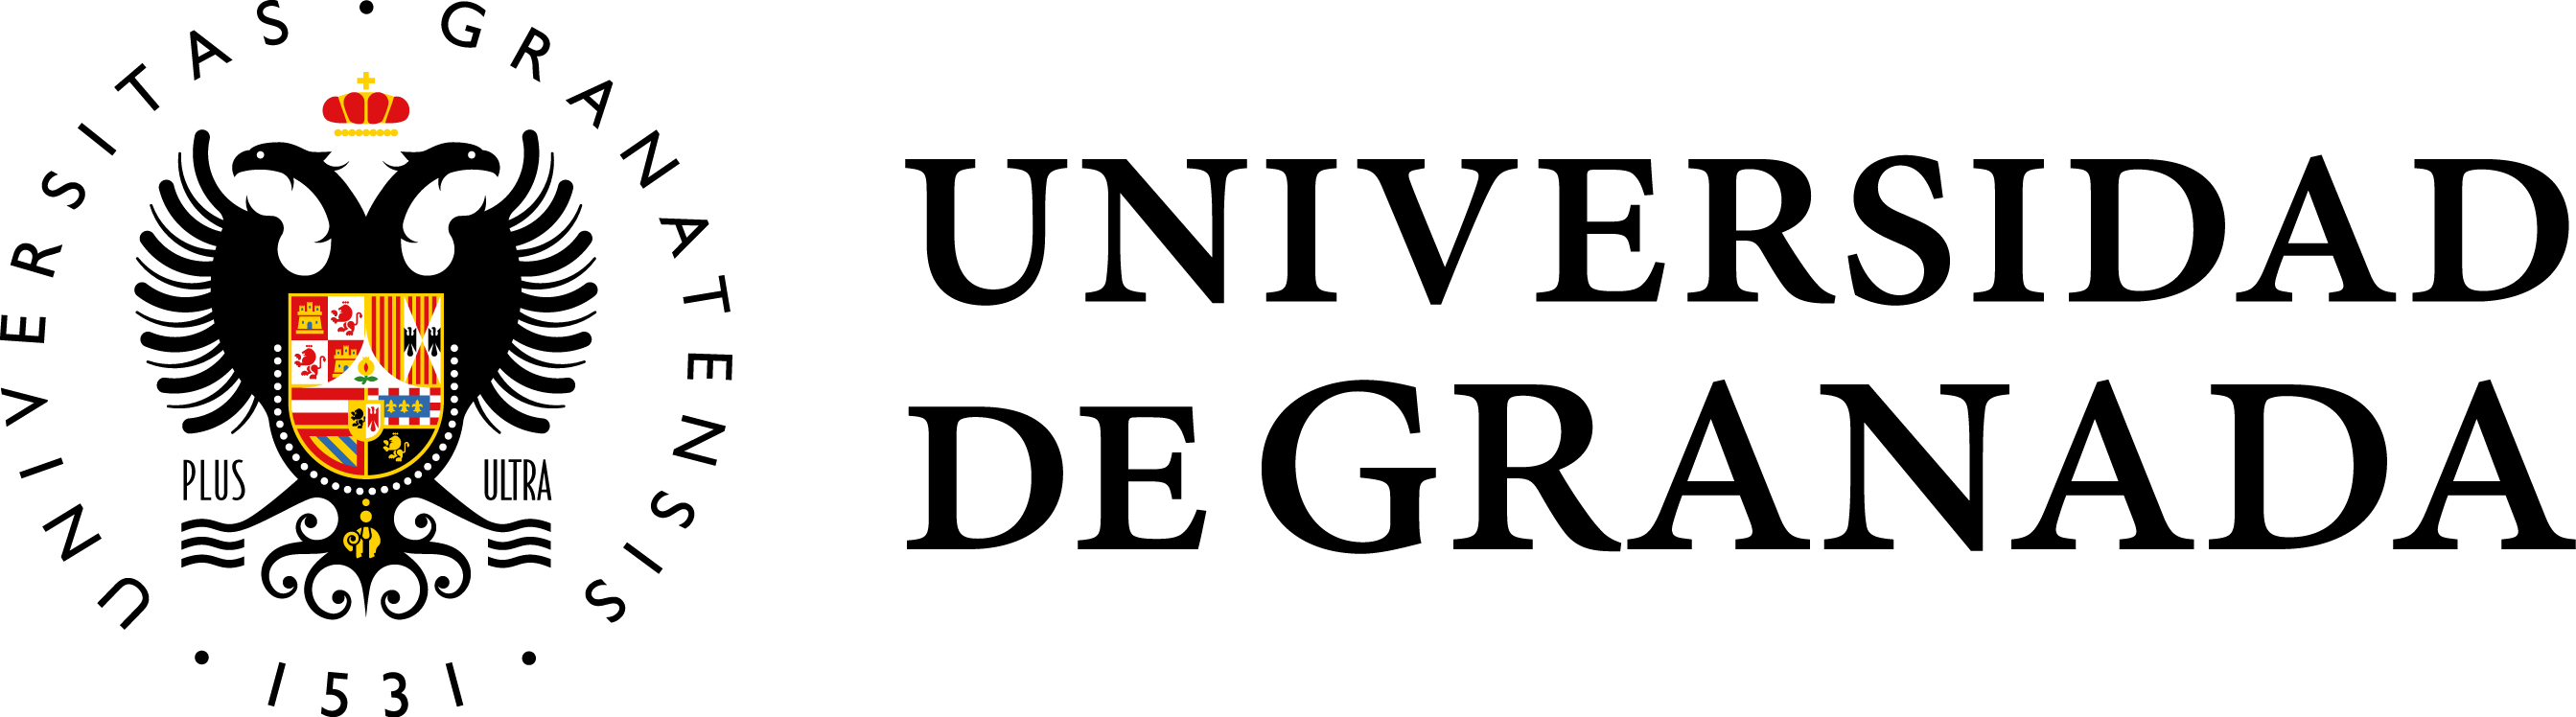
\includegraphics[width=0.25\textwidth]{../../../extraFiles/img/ugr.png} % opcional: logo
        % \vspace{1cm}
        
        % {\large \today}
    \end{center}
    
    \restoregeometry
\end{titlepage}


% ===============================
% licencia.tex
% ===============================
\section*{Licencia}

Este trabajo está licenciado bajo una 
\href{https://creativecommons.org/licenses/by-nc-nd/4.0/}{Licencia Creative Commons Reconocimiento-NoComercial-SinObraDerivada 4.0 Internacional}.

\bigskip

\textbf{Usted es libre de:}
\begin{itemize}
  \item \textbf{Compartir} — copiar y redistribuir el material en cualquier medio o formato.
\end{itemize}

\bigskip

\textbf{Bajo los siguientes términos:}
\begin{description}
  \item[\textbf{Reconocimiento}] Debe otorgar el crédito adecuado, proporcionar un enlace a la licencia e indicar si se han realizado cambios. Puede hacerlo de cualquier manera razonable, pero no de una manera que sugiera que tiene el apoyo del licenciante o lo recibe por el uso que hace.

  \item[\textbf{NoComercial}] No puede utilizar el material para fines comerciales.

  \item[\textbf{SinObraDerivada}] Si remezcla, transforma o crea a partir del material, no puede distribuir el material modificado.
\end{description}

\bigskip

\begin{center}
  \href{https://creativecommons.org/licenses/by-nc-nd/4.0/}{
\includegraphics[width=0.35\textwidth]{../../../extraFiles/img/by-nc-nd.png}}
\end{center}
  % licencia
\thispagestyle{empty} % quitar número de página en la portada
\clearpage

% --- Índice ---
\tableofcontents
% \listoffigures
\clearpage

%\listoftables
%\clearpage
%\thispagestyle{empty} % quitar número de página en la portada
%\clearpage
%
% Índice de código
%\renewcommand{\lstlistlistingname}{Índice de Código}
%\lstlistoflistings
%\clearpage
%
% Índice de ecuaciones
%\renewcommand{\listtheoremname}{Índice de Ecuaciones}
%\listoftheorems[ignoreall,show={equation}]
%\clearpage

% --- Contenido Markdown generado por Pandoc ---
\part{Teoría}

\hypertarget{introducciuxf3n}{%
\chapter{Introducción}\label{introducciuxf3n}}

\begin{itemize}
\tightlist
\item
  Profesor: Serafín Moral\\
\item
  Correo: smc@decsai.ugr.es\\
\item
  El profesor recomienda ir a las tutorías y avisarle antes.\\
\item
  J.E. Hopcroft, J.D. Ullman, Introduction to Automata Theory, Languages
  and Computation. Addison-Wesley (1979): un libro básico, se requiere
  ciertos conocimientos matemáticos para leerlo.\\
\item
  M. Alfonseca, J. Sancho. M. Martínez, Teoría de Autómatas y Lenguajes
  Formales. Publicaciones R.A.E.C., Textos Cátedra (1997): básico y
  fácil de entender, está en la biblioteca en español.\\
\item
  Los demás son una buena opción también.
\end{itemize}

La asignatura de Modelos de Computación se centra en el estudio de los
fundamentos teóricos de la informática, explorando conceptos como
autómatas, lenguajes formales, gramáticas y máquinas de Turing. Estos
temas proporcionan las bases para comprender las capacidades y
limitaciones de los sistemas computacionales, así como para analizar la
complejidad de los problemas y los algoritmos que los resuelven. Es una
materia esencial para quienes deseen profundizar en la teoría de la
computación y su aplicación en el diseño de sistemas eficientes y
correctos.

\hypertarget{introducciuxf3n-a-la-computaciuxf3n}{%
\chapter{Introducción a la
Computación}\label{introducciuxf3n-a-la-computaciuxf3n}}

En el pasado, había teoremas que eran verdad, pero las matemáticas no
eran capaces de demostrarlo. Turing puso solución a esto exponiendo que
esta incompletitud de las matemáticas se corregía diciendo que este tipo
de problemas eran indecidibles. En cuanto a la complejidad de los
algoritmos, como vimos en algorítmica, podemos distinguir entre p
(polinómico) y np (polinómico no determinista). Dentro de np,
encontramos los np completos y los np difíciles (problemas que no puede
resolver un ordenador convencional). Hoy día lo más importante es la
complejidad algorítmica. Nadie ha demostrado que p sea distinto de np.

\hypertarget{problema-de-la-parada}{%
\section{Problema de la parada}\label{problema-de-la-parada}}

Trata el tema de la existencia de que un programa que lea otro programa
y unos datos y nos diga si este termina o cicla indefinidamente. Un
programa es lo mismo que los datos, según Turing. En este caso, se pone
como datos del programa el mismo programa.

\begin{lstlisting}[language=Python]
If Stops(P, P) GOTO L
\end{lstlisting}

Este programa lleva a una contradicción, ya que si termina no termina y
si termina termina, cosa que no es coherente. Por ende, podemos concluir
que si un programa se llama así mismo, en este caso, llegamos a una
contradicción. Turing, con esto, llegó a la conclusión de que las
matemáticas eran incompletas, ya que este programa no existe. La
explicación es sencilla, basta con decir que es como un espejo, nunca va
a pasar STOP ya que si eso pasa el programa nunca arrancaría.

\hypertarget{definiciones}{%
\section{Definiciones}\label{definiciones}}

\begin{definicion}
\textbf{Alfabeto}: Un alfabeto es un conjunto finito cuyos elementos se denominan símbolos o letras. Si los símbolos tienen varios elementos, se representan entre $\langle \rangle$.  
\end{definicion}

\begin{definicion}
\textbf{Palabra}: Una palabra es una sucesión finita de elementos de un alfabeto $A$. Formalmente, $u = a_1 a_2 \ldots a_n$, donde $a_i \in A$ para todo $i = 1, \ldots, n$.  
\end{definicion}

\begin{definicion}
\textbf{Conjunto de Palabras}: El conjunto de todas las palabras que se pueden formar sobre un alfabeto $A$ se denota como $A^*$.  
\end{definicion}

\begin{definicion}
\textbf{Notación de Palabras}: Las palabras se denotan comúnmente como $u, v, x, y, z, \ldots$.  
\end{definicion}

\begin{definicion}
\textbf{Longitud de una Palabra}: Si $u \in A^*$, la longitud de la palabra $u$ es el número de símbolos de $A$ que contiene.  
\begin{itemize}
    \item Notación: $\lvert u \rvert$  
    \item Si $u = a_1 a_2 \ldots a_n$, entonces $\lvert u \rvert = n$.  
\end{itemize}
\end{definicion}

\begin{definicion}
\textbf{Palabra Vacía}: La palabra vacía es la palabra de longitud cero.  
\begin{itemize}
    \item Notación: $\varepsilon$  
\end{itemize}
\end{definicion}

\begin{definicion}
\textbf{Conjunto de Palabras no Vacías}: El conjunto de cadenas sobre un alfabeto $A$ excluyendo la palabra vacía se denota como $A^+$.  
\end{definicion}

\hypertarget{operaciones-concatenaciuxf3n}{%
\section{Operaciones:
Concatenación}\label{operaciones-concatenaciuxf3n}}

\begin{definicion}
\textbf{Concatenación de Palabras}: Si $u, v \in A^*$, $u = a_1 \ldots a_n$, $v = b_1 \ldots b_m$, se llama concatenación de $u$ y $v$ a la cadena $u.v$ (o simplemente $uv$) dada por $a_1 \ldots a_n b_1 \ldots b_m$.
\end{definicion}

\begin{ejemplo}
Si $u = 011$, $v = 1010$, entonces $uv = 0111010$.
\end{ejemplo}

\textbf{Propiedades}

\begin{enumerate}
\def\labelenumi{\arabic{enumi}.}
\tightlist
\item
  \(\lvert u.v \rvert = \lvert u \rvert + \lvert v \rvert\),
  \(\forall u, v \in A^*\)\\
\item
  \textbf{Asociativa}: \(u.(v.w) = (u.v).w\),
  \(\forall u, v, w \in A^*\)\\
\item
  \textbf{Elemento Neutro}: \(u.\varepsilon = \varepsilon.u = u\),
  \(\forall u \in A^*\)
\end{enumerate}

\begin{definicion}
\textbf{Monoide}: Un monoide es una estructura algebraica $(M, \cdot, e)$ que consta de un conjunto $M$, una operación binaria asociativa $\cdot : M \times M \to M$, y un elemento neutro $e \in M$ tal que:  
1. Asociatividad: $(a \cdot b) \cdot c = a \cdot (b \cdot c)$, $\forall a, b, c \in M$.  
2. Elemento Neutro: $a \cdot e = e \cdot a = a$, $\forall a \in M$.  
\end{definicion}

\textbf{Estructura de monoide}\\
La concatenación de palabras sobre un alfabeto \(A\) junto con la
palabra vacía \(\varepsilon\) forma un monoide.

\hypertarget{prefijos-sufijos-y-subcadenas}{%
\section{Prefijos, Sufijos y
subcadenas}\label{prefijos-sufijos-y-subcadenas}}

\begin{definicion}
\textbf{Prefijo}: Si $u \in A^*$, entonces $v$ es un prefijo de $u$ si $\exists z \in A^*$ tal que $vz = u$.  
Un prefijo $v$ de $u$ se dice propio si $v \neq \varepsilon$ y $v \neq u$.  
\end{definicion}

\begin{definicion}
\textbf{Sufijo}: Si $u \in A^*$, entonces $v$ es un sufijo de $u$ si $\exists z \in A^*$ tal que $zv = u$.  
Un sufijo $v$ de $u$ se dice propio si $v \neq \varepsilon$ y $v \neq u$.  
\end{definicion}

\begin{definicion}
\textbf{Subcadena}: Si $u \in A^*$, entonces $v$ es una subcadena de $u$ si $\exists z_1, z_2 \in A^*$ tal que $z_1vz_2 = u$.  
Una subcadena $v$ de $u$ se dice propia si $v \neq \varepsilon$ y $v \neq u$.  
\end{definicion}

\hypertarget{iteraciuxf3n-y-palabra-inversa}{%
\section{Iteración y Palabra
Inversa}\label{iteraciuxf3n-y-palabra-inversa}}

\begin{definicion}
\textbf{Iteración de una Cadena}: La iteración n-ésima de una cadena ($u^n$) se define como la concatenación de la cadena consigo misma $n$ veces.  
Si $u \in A^*$, entonces:  
\begin{itemize}
    \item $u^0 = \varepsilon$  
    \item $u^{i+1} = u^i.u$, $\forall i \geq 0$  
\end{itemize}
\end{definicion}

\begin{ejemplo}
Si $u = 010$, entonces $u^3 = 010010010$.
\end{ejemplo}

\begin{definicion}
\textbf{Palabra Inversa}: Si $u = a_1 \ldots a_n \in A^*$, entonces la palabra inversa de $u$ es la cadena $u^{-1} = a_n \ldots a_1 \in A^*$.  
\end{definicion}

\begin{ejemplo}
Si $u = 011$, entonces la palabra inversa de $u$ es $u^{-1} = 110$.
\end{ejemplo}

\hypertarget{lenguajes}{%
\section{Lenguajes}\label{lenguajes}}

\begin{definicion}
\textbf{Lenguaje}: Un lenguaje sobre un alfabeto $A$ es un subconjunto del conjunto de las cadenas sobre $A$, es decir, $L \subseteq A^*$.  
La palabra vacía siempre pertenece a un lenguaje.
\end{definicion}

\textbf{Notación}\\

\begin{itemize}
    \item Lenguajes: $L, M, N, \ldots$
\end{itemize}

\begin{ejemplo}
    \begin{enumerate}
        \item $L_1 = \{a, b, \varepsilon\}$  
        \item $L_2 = \{a^i b^i \mid i = 0, 1, 2, \ldots\}$  
        \item $L_3 = \{u u^{-1} \mid u \in A^*\}$  
        \item $L_4 = \{a^{n^2} \mid n = 1, 2, 3, \ldots\}$  
    \end{enumerate}
\end{ejemplo}

\hypertarget{ejemplos-adicionales-de-lenguajes}{%
\subsection{Ejemplos Adicionales de
Lenguajes}\label{ejemplos-adicionales-de-lenguajes}}

\begin{enumerate}
\def\labelenumi{\arabic{enumi}.}
\tightlist
\item
  \(L_5 = \{a^n b^m c^k \mid n, m, k \geq 0\}\): Palabras con cualquier
  número de \(a\), \(b\), y \(c\) en ese orden.\\
\item
  \(L_6 = \{w \in \{0, 1\}^* \mid w \text{ tiene un número par de } 1\}\):
  Palabras binarias con un número par de unos.\\
\item
  \(L_7 = \{a^n b^n c^n \mid n \geq 0\}\): Palabras con el mismo número
  de \(a\), \(b\), y \(c\) en ese orden.\\
\item
  \(L_8 = \{w \in \{0, 1\}^* \mid w \text{ es un palíndromo}\}\):
  Palabras binarias que son palíndromos.\\
\item
  \(L_9 = \{a^{2^n} \mid n \geq 0\}\): Sucesiones de \(a\) cuya longitud
  es una potencia de dos.
\end{enumerate}

\hypertarget{conjuntos-numerables}{%
\subsection{Conjuntos Numerables}\label{conjuntos-numerables}}

Un conjunto se dice numerable si existe una aplicación inyectiva
(corresponde cada elemento con su imagen) de este conjunto en el
conjunto de los números naturales, o lo que es lo mismo, se le puede
asignar un número natural a cada elemento del conjunto de tal manera que
dos elementos distintos tengan números distintos.

\begin{ejemplo}
$A^*$ es siempre numerable. Si $A = \{a_1, \ldots, a_n\}$, entonces puedo asignar un número binario distinto de 0 y de la misma longitud a cada $a_i$ de tal manera que símbolos distintos reciben números distintos, y a cada palabra $b_1 \ldots b_k$ se le asigna el número cuya representación en binario es el que se obtiene sustituyendo cada $b_i$ por su número binario.  

\textit{Ejemplo}: Si $A = \{a, b\}$, podemos asignar $a = 01$, $b = 10$. Entonces, para la palabra $ab$, su representación binaria sería $0110$.  
\end{ejemplo}

\begin{ejemplo}
El conjunto de programas bien escritos en C es numerable. Esto se debe a que los programas son cadenas finitas de un alfabeto finito, y por lo tanto, se pueden enumerar de manera similar a las palabras en $A^*$.  
\end{ejemplo}

El hecho de que en el ordenador se trabaje con float, double, \ldots{}
es porque como los números reales son conjuntos no numerables, un solo
número real acabaría con toda la memoria del ordenador. Lo mismo pasa en
los lenguajes, debemos de restringirnos a los lenguajes con los que
podamos trabajar. Solo existe un conjunto numerable de programas.

\hypertarget{un-conjunto-no-numerable}{%
\section{Un Conjunto No Numerable}\label{un-conjunto-no-numerable}}

\begin{ejemplo}
El conjunto de lenguajes sobre $A^*$ (si $A$ no es vacío) nunca es numerable.  
\end{ejemplo}

Haremos la demostración por reducción al absurdo.\\

\begin{demostracion}
Si lo fuese, se podría asignar un número natural distinto $f(L)$ a cada lenguaje $L$.  

Sea $a \in A$.  
Definamos el lenguaje $L$ formado por palabras de la forma $a^i$ de acuerdo a lo siguiente: para cada $i$ número natural:  
\begin{itemize}
    \item Si este número no es de un lenguaje, entonces $a^i \in L$.  
    \item Si este número es del lenguaje $M$ ($i = f(M)$):  
        \begin{itemize}
            \item Si $a^i \notin M$, entonces $a^i \in L$.  
            \item Si $a^i \in M$, entonces $a^i \notin L$.  
        \end{itemize}
\end{itemize}

$L$ no puede tener ningún número asociado. Si fuese $j = f(L)$, entonces la pertenencia de $a^j$ a $L$ es contradictoria:  
\begin{itemize}
    \item Si $a^j \in L$ como $j = f(L)$, entonces $a^j \notin L$.  
    \item Si $a^j \notin L$ y $j = f(L)$, entonces $a^j \in L$.  
\end{itemize}

Por lo tanto, el conjunto de lenguajes sobre $A^*$ no es numerable.  
\end{demostracion}

\hypertarget{operaciones-con-lenguajes-concatenaciuxf3n}{%
\section{Operaciones con Lenguajes:
Concatenación}\label{operaciones-con-lenguajes-concatenaciuxf3n}}

Dada su condición de conjuntos, además de las operaciones de unión,
intersección y complementario, los lenguajes también admiten la
operación de concatenación.

Si \(L_1, L_2\) son dos lenguajes sobre el alfabeto \(A\), la
concatenación de estos dos lenguajes se define como:

\[
L_1L_2 = \{u_1u_2 \mid u_1 \in L_1, u_2 \in L_2\}
\]

\begin{ejemplo}
Si $L_1 = \{0^i1^i \mid i \geq 0\}$ y $L_2 = \{1^j0^j \mid j \geq 0\}$, entonces:

$$
L_1L_2 = \{0^i1^i1^j0^j \mid i, j \geq 0\}
$$
\end{ejemplo}

\hypertarget{propiedades-de-la-concatenaciuxf3n-de-lenguajes}{%
\section{Propiedades de la Concatenación de
Lenguajes}\label{propiedades-de-la-concatenaciuxf3n-de-lenguajes}}

\begin{enumerate}
\def\labelenumi{\arabic{enumi}.}
\item
  \textbf{Propiedad de Aniquilación}\\
  \[L \emptyset = \emptyset L = \emptyset\]
\item
  \textbf{Elemento Neutro}\\
  \[\{\varepsilon\}L = L\{\varepsilon\} = L\]
\item
  \textbf{Asociatividad}\\
  \[L_1(L_2L_3) = (L_1L_2)L_3\]
\end{enumerate}

\hypertarget{iteraciuxf3n-de-lenguajes-y-clausura-de-kleene}{%
\section{Iteración de Lenguajes y Clausura de
Kleene}\label{iteraciuxf3n-de-lenguajes-y-clausura-de-kleene}}

La iteración de lenguajes se define de forma recursiva:

\begin{itemize}
\tightlist
\item
  \(L^0 = \{\varepsilon\}\)\\
\item
  \(L^{i+1} = L^iL\), \(\forall i \geq 0\)
\end{itemize}

Si \(L\) es un lenguaje sobre el alfabeto \(A\), se definen las
siguientes clausuras:

\begin{itemize}
\item
  \textbf{Clausura de Kleene}:\\
  \[
    L^* = \bigcup_{i \geq 0} L^i
    \]
\item
  \textbf{Clausura Positiva}:\\
  \[
    L^+ = \bigcup_{i \geq 1} L^i
    \]
\end{itemize}

\begin{ejemplo}
Si $L = \{a, b\}$:  
\begin{itemize}
    \item $L^0 = \{\varepsilon\}$  
    \item $L^1 = \{a, b\}$  
    \item $L^2 = \{aa, ab, ba, bb\}$  
    \item $L^* = \{\varepsilon, a, b, aa, ab, ba, bb, \ldots\}$  
    \item $L^+ = \{a, b, aa, ab, ba, bb, \ldots\}$  
\end{itemize}
\end{ejemplo}

\hypertarget{operaciones-con-lenguajes-propiedades-de-clausuras}{%
\section{Operaciones con Lenguajes: Propiedades de
Clausuras}\label{operaciones-con-lenguajes-propiedades-de-clausuras}}

\begin{enumerate}
\def\labelenumi{\arabic{enumi}.}
\tightlist
\item
  \textbf{Relación entre Clausura de Kleene y Clausura Positiva}

  \begin{itemize}
  \tightlist
  \item
    Si \(\varepsilon \in L\), entonces \(L^+ = L^*\).\\
  \item
    Si \(\varepsilon \notin L\), entonces
    \(L^+ = L^* \setminus \{\varepsilon\}\).
  \end{itemize}
\end{enumerate}

\begin{ejemplo}
Si $L = \{0, 01\}$:  
    \begin{itemize}
        \item $L^* =$ Conjunto de palabras sobre $\{0, 1\}$ en las que un $1$ siempre va precedido de un $0$.  
        \item $L^+ =$ Conjunto de palabras sobre $\{0, 1\}$ en las que un $1$ siempre va precedido de un $0$ y distintas de la palabra vacía.  
    \end{itemize}
\end{ejemplo}

\hypertarget{lenguaje-inverso}{%
\section{Lenguaje Inverso}\label{lenguaje-inverso}}

\begin{definicion}
\textbf{Lenguaje Inverso}: El lenguaje inverso de un lenguaje $L$ sobre un alfabeto $A$ se define como:

$$
L^{-1} = \{u \mid u^{-1} \in L\}
$$
\end{definicion}

\begin{ejemplo}
Si $L = \{011, 101\}$, entonces:

$$
L^{-1} = \{110, 101\}
$$
\end{ejemplo}

\textbf{Propiedades}

\begin{enumerate}
\def\labelenumi{\arabic{enumi}.}
\tightlist
\item
  \((L^{-1})^{-1} = L\)\\
\item
  \((L_1 \cup L_2)^{-1} = L_1^{-1} \cup L_2^{-1}\)\\
\item
  \((L_1L_2)^{-1} = L_2^{-1}L_1^{-1}\)\\
\item
  \((L^*)^{-1} = (L^{-1})^*\)
\end{enumerate}

\hypertarget{cabecera-de-un-lenguaje}{%
\section{Cabecera de un Lenguaje}\label{cabecera-de-un-lenguaje}}

\begin{definicion}
\textbf{Cabecera de un Lenguaje}: La cabecera de un lenguaje $L$ sobre un alfabeto $A$ se define como:

$$
\text{CAB}(L) = \{u \mid u \in A^* \text{ y } \exists v \in A^* \text{ tal que } uv \in L\}
$$
\end{definicion}

\begin{ejemplo}
Si $L = \{0^i1^i \mid i \geq 0\}$, entonces:

$$
\text{CAB}(L) = \{0^i1^j \mid i \geq j \geq 0\}
$$
\end{ejemplo}

\hypertarget{homomorfismos-entre-alfabetos}{%
\section{Homomorfismos entre
Alfabetos}\label{homomorfismos-entre-alfabetos}}

\begin{definicion}
Si $A_1$ y $A_2$ son dos alfabetos, una aplicación $h : A_1^* \to A_2^*$ se dice que es un \textbf{homomorfismo} si y solo si:

$$
h(uv) = h(u)h(v), \quad \forall u, v \in A_1^*
$$

La transformación de uv debe de ser igual a la concatenación de la transformación de u y la transformación de v.
\end{definicion}

\hypertarget{consecuencias-de-la-definiciuxf3n}{%
\subsection{Consecuencias de la
Definición}\label{consecuencias-de-la-definiciuxf3n}}

\begin{enumerate}
\def\labelenumi{\arabic{enumi}.}
\item
  \textbf{Imagen de la palabra vacía}\\
  \[
   h(\varepsilon) = \varepsilon
   \]
\item
  \textbf{Imagen de una palabra}\\
  Si \(u = a_1a_2 \ldots a_n \in A_1^*\), entonces: \[
   h(u) = h(a_1)h(a_2) \ldots h(a_n)
   \]
\end{enumerate}

\begin{ejemplo}
    \textbf{Ejemplo de Homomorfismo}

    Sea $A_1 = \{a, b\}$ y $A_2 = \{0, 1\}$. Definimos $h : A_1^* \to A_2^*$ como:

    \begin{itemize}
        \item $h(a) = 01$
        \item $h(b) = 10$
    \end{itemize}

    Entonces:

    \begin{itemize}
        \item $h(\varepsilon) = \varepsilon$
        \item $h(ab) = h(a)h(b) = 0110$
        \item $h(aba) = h(a)h(b)h(a) = 010110$
    \end{itemize}
\end{ejemplo}

\hypertarget{propiedades-de-homomorfismos}{%
\subsection{Propiedades de
Homomorfismos}\label{propiedades-de-homomorfismos}}

\begin{enumerate}
\def\labelenumi{\arabic{enumi}.}
\item
  \textbf{Preservación de la Concatenación}\\
  \[
   h(u.v) = h(u)h(v), \quad \forall u, v \in A_1^*
   \]
\item
  \textbf{Homomorfismo Inverso}\\
  Si \(h : A_1^* \to A_2^*\) es un homomorfismo, entonces: \[
   h(u^{-1}) = h(u)^{-1}, \quad \forall u \in A_1^*
   \]
\item
  \textbf{Composición de Homomorfismos}\\
  Si \(h_1 : A_1^* \to A_2^*\) y \(h_2 : A_2^* \to A_3^*\) son
  homomorfismos, entonces su composición
  \(h_2 \circ h_1 : A_1^* \to A_3^*\) también es un homomorfismo.
\end{enumerate}

\begin{ejemplo}
    \textbf{Ejemplo de Composición}  
    Sea $h_1 : A_1^* \to A_2^*$ y $h_2 : A_2^* \to A_3^*$ definidos como:

    \begin{itemize}
        \item $h_1(a) = 01$
        \item $h_1(b) = 10$
        \item $h_2(0) = x$
        \item $h_2(1) = y$
    \end{itemize}

    Entonces, para $u = ab \in A_1^*$:

    \begin{itemize}
        \item $h_1(u) = 0110$
        \item $h_2(h_1(u)) = h_2(0110) = xyxy$
    \end{itemize}
\end{ejemplo}

\hypertarget{gramuxe1tica-generativa}{%
\section{Gramática Generativa}\label{gramuxe1tica-generativa}}

\begin{definicion}
Una gramática generativa es una cuádrupla $(V, T, P, S)$ donde:

\begin{itemize}
    \item \textbf{$V$}: Es un alfabeto llamado de variables o símbolos no terminales. Sus elementos se suelen representar con letras mayúsculas.
    \item \textbf{$T$}: Es un alfabeto llamado de símbolos terminales. Sus elementos se suelen representar con letras minúsculas.
    \item \textbf{$P$}: Es un conjunto finito de pares $(\alpha, \beta)$, llamados reglas de producción, donde $\alpha, \beta \in (V \cup T)^*$ y $\alpha$ contiene al menos un símbolo de $V$.
        \begin{itemize}
            \item El par $(\alpha, \beta)$ se suele representar como $\alpha \to \beta$.
        \end{itemize}
    \item \textbf{$S$}: Es un elemento de $V$, llamado símbolo de partida.
\end{itemize}
\end{definicion}

Tiene la misma potencia que un lenguaje, por ende, podemos pensar que es
similar a un lenguaje de programación aunque pensemos que no.

\begin{ejemplo}
Sea la gramática $G = (V, T, P, S)$ definida como:  
    \begin{itemize}
        \item $V = \{S, A\}$  
        \item $T = \{a, b\}$  
        \item $P = \{S \to aA, A \to b\}$  
        \item $S = S$  
    \end{itemize}
\end{ejemplo}

Esta gramática genera el lenguaje \(L = \{ab\}\).

\hypertarget{lenguaje-generado-idea-intuitiva}{%
\section{Lenguaje Generado: Idea
Intuitiva}\label{lenguaje-generado-idea-intuitiva}}

Una gramática sirve para determinar un lenguaje. Las palabras generadas
pertenecen al conjunto de símbolos terminales \(T^*\) y se obtienen a
partir del símbolo inicial efectuando pasos de derivación. Cada paso
consiste en elegir una parte de la palabra que coincide con la parte
izquierda de una producción y sustituir esa parte por la derecha de la
misma producción.

\begin{ejemplo}
    Dada la gramática:

    \begin{itemize}
        \item $E \to E + E$
        \item $E \to E * E$
        \item $E \to (E)$
        \item $E \to a$
        \item $E \to b$
        \item $E \to c$
    \end{itemize}

    Derivación de una palabra:

    $$
    E \Rightarrow E * E \Rightarrow (E) * E \Rightarrow (E + E) * E \Rightarrow (a + E) * E \Rightarrow (a + b) * E \Rightarrow (a + b) * b
    $$

    \textbf{Palabra Generada}: $(a + b) * b$
\end{ejemplo}

\hypertarget{derivaciuxf3n-y-lenguaje-generado}{%
\section{Derivación y Lenguaje
Generado}\label{derivaciuxf3n-y-lenguaje-generado}}

\hypertarget{derivaciuxf3n-en-un-paso}{%
\subsection{Derivación en un Paso}\label{derivaciuxf3n-en-un-paso}}

Dada una gramática \(G = (V, T, P, S)\) y dos palabras
\(\alpha, \beta \in (V \cup T)^*\), se dice que \(\beta\) es derivable a
partir de \(\alpha\) en un paso (\(\alpha \Rightarrow \beta\)) si y solo
si existe una producción \(\gamma \to \phi\) tal que \(\alpha\) contiene
a \(\gamma\) como subcadena y \(\beta\) se obtiene sustituyendo
\(\gamma\) por \(\phi\) en \(\alpha\).

\hypertarget{secuencia-de-derivaciuxf3n}{%
\subsection{Secuencia de Derivación}\label{secuencia-de-derivaciuxf3n}}

Se dice que \(\beta\) es derivable de \(\alpha\)
(\(\alpha \overset{*}{\Rightarrow} \beta\)) si y solo si existe una
sucesión de palabras \(\gamma_1, \ldots, \gamma_n\) (\(n \geq 1\)) tales
que:

\[
\alpha = \gamma_1 \Rightarrow \gamma_2 \Rightarrow \ldots \Rightarrow \gamma_n = \beta
\]

\hypertarget{lenguaje-generado-por-una-gramuxe1tica}{%
\subsection{Lenguaje Generado por una
Gramática}\label{lenguaje-generado-por-una-gramuxe1tica}}

El lenguaje generado por una gramática \(G = (V, T, P, S)\) es el
conjunto de cadenas formadas por símbolos terminales que son derivables
a partir del símbolo de partida \(S\). Formalmente:

\[
L(G) = \{u \in T^* \mid S \overset{*}{\Rightarrow} u\}
\]

\hypertarget{gramuxe1tica-generativa-ejemplo-y-propiedades}{%
\section{Gramática Generativa: Ejemplo y
Propiedades}\label{gramuxe1tica-generativa-ejemplo-y-propiedades}}

\hypertarget{gramuxe1tica-definida}{%
\subsection{Gramática Definida}\label{gramuxe1tica-definida}}

Sea la gramática \(G = (V, T, P, S)\) definida como:\\
- \(V = \{S, A, B\}\)\\
- \(T = \{a, b\}\)\\
-
\(P = \{S \to aB, S \to bA, A \to a, A \to aS, A \to bAA, B \to b, B \to bS, B \to aBB\}\)\\
- \(S = S\)

\hypertarget{lenguaje-generado}{%
\subsection{Lenguaje Generado}\label{lenguaje-generado}}

Esta gramática genera el lenguaje:

\[
L(G) = \{u \mid u \in \{a, b\}^+ \text{ y } N_a(u) = N_b(u)\}
\]

donde \(N_a(u)\) y \(N_b(u)\) son el número de apariciones de los
símbolos \(a\) y \(b\) en \(u\), respectivamente.

\hypertarget{interpretaciuxf3n-de-las-variables}{%
\subsection{Interpretación de las
Variables}\label{interpretaciuxf3n-de-las-variables}}

\begin{itemize}
\tightlist
\item
  \(A\): Representa palabras con una \(a\) de más.\\
\item
  \(B\): Representa palabras con una \(b\) de más.\\
\item
  \(S\): Representa palabras con igual número de \(a\) que de \(b\).
\end{itemize}

\hypertarget{propiedades-del-lenguaje-generado}{%
\subsection{Propiedades del Lenguaje
Generado}\label{propiedades-del-lenguaje-generado}}

\begin{enumerate}
\def\labelenumi{\arabic{enumi}.}
\tightlist
\item
  \textbf{Todas las palabras generadas tienen el mismo número de \(a\)
  que de \(b\).}\\
\item
  \textbf{Cualquier palabra con el mismo número de \(a\) que de \(b\)
  puede ser generada.}
\end{enumerate}

\hypertarget{demostraciuxf3n-de-la-primera-propiedad}{%
\subsection{Demostración de la Primera
Propiedad}\label{demostraciuxf3n-de-la-primera-propiedad}}

\begin{demostracion}
Consideremos $N_{a,A}(\alpha)$ (número de $a$ más número de $A$) y $N_{b,B}(\alpha)$ (número de $b$ más número de $B$). Para una derivación $S \overset{*}{\Rightarrow} u$, tenemos:  

\begin{itemize}
    \item Al inicio: $N_{a,A}(S) = N_{b,B}(S) = 0$.  
    \item Al aplicar cualquier regla $\alpha_1 \to \alpha_2$, si $N_{a,A}(\alpha_1) = N_{b,B}(\alpha_1)$, entonces $N_{a,A}(\alpha_2) = N_{b,B}(\alpha_2)$.  
\end{itemize}

Por lo tanto, al final de la derivación, $N_{a,A}(u) = N_{b,B}(u)$. Como $u$ no contiene variables, $N_a(u) = N_b(u)$, lo que demuestra la propiedad.
\end{demostracion}

\hypertarget{algoritmo-de-generaciuxf3n}{%
\subsection{Algoritmo de Generación}\label{algoritmo-de-generaciuxf3n}}

La generación de palabras se realiza por la izquierda, un símbolo a la
vez:

\begin{itemize}
\tightlist
\item
  \textbf{Para generar una \(a\):}

  \begin{itemize}
  \tightlist
  \item
    Si \(a\) es el último símbolo, aplicar \(A \to a\).\\
  \item
    Si no es el último símbolo:

    \begin{itemize}
    \tightlist
    \item
      Si la primera variable es \(S\), aplicar \(S \to aB\).\\
    \item
      Si la primera variable es \(B\), aplicar \(B \to aBB\).\\
    \item
      Si la primera variable es \(A\):

      \begin{itemize}
      \tightlist
      \item
        Si hay más variables, aplicar \(A \to a\).\\
      \item
        Si no hay más, aplicar \(A \to aS\).
      \end{itemize}
    \end{itemize}
  \end{itemize}
\item
  \textbf{Para generar una \(b\):}

  \begin{itemize}
  \tightlist
  \item
    Si \(b\) es el último símbolo, aplicar \(B \to b\).\\
  \item
    Si no es el último símbolo:

    \begin{itemize}
    \tightlist
    \item
      Si la primera variable es \(S\), aplicar \(S \to bA\).\\
    \item
      Si la primera variable es \(A\), aplicar \(A \to bAA\).\\
    \item
      Si la primera variable es \(B\):

      \begin{itemize}
      \tightlist
      \item
        Si hay más variables, aplicar \(B \to b\).\\
      \item
        Si no hay más, aplicar \(B \to bS\).
      \end{itemize}
    \end{itemize}
  \end{itemize}
\end{itemize}

\hypertarget{condiciones-de-garantuxeda}{%
\subsection{Condiciones de Garantía}\label{condiciones-de-garantuxeda}}

\begin{enumerate}
\def\labelenumi{\arabic{enumi}.}
\tightlist
\item
  Las palabras generadas tienen primero símbolos terminales y después
  variables.\\
\item
  Se genera un símbolo de la palabra en cada paso de derivación.\\
\item
  Las variables que aparecen en la palabra pueden ser:

  \begin{itemize}
  \tightlist
  \item
    Una cadena de \(A\) (si se han generado más \(b\) que \(a\)).\\
  \item
    Una cadena de \(B\) (si se han generado más \(a\) que \(b\)).\\
  \item
    Una \(S\) (si se han generado el mismo número de \(a\) y \(b\)).
  \end{itemize}
\end{enumerate}

Antes de generar el último símbolo, las variables serán:\\
- Una \(A\) si se necesita generar una \(a\).\\
- Una \(B\) si se necesita generar una \(b\).

En este caso, se aplica la primera opción para generar los símbolos, y
la palabra queda generada.

\hypertarget{gramuxe1tica-alternativa-para-el-mismo-lenguaje}{%
\section{Gramática Alternativa para el Mismo
Lenguaje}\label{gramuxe1tica-alternativa-para-el-mismo-lenguaje}}

\hypertarget{gramuxe1tica-que-incluye-la-palabra-vacuxeda}{%
\subsection{Gramática que Incluye la Palabra
Vacía}\label{gramuxe1tica-que-incluye-la-palabra-vacuxeda}}

Esta gramática genera todas las palabras con el mismo número de símbolos
\(a\) que \(b\), incluyendo la palabra vacía:

\begin{itemize}
\tightlist
\item
  \(S \to aSbS\)
\item
  \(S \to bSaS\)
\item
  \(S \to \varepsilon\)
\end{itemize}

\hypertarget{gramuxe1tica-que-excluye-la-palabra-vacuxeda}{%
\subsection{Gramática que Excluye la Palabra
Vacía}\label{gramuxe1tica-que-excluye-la-palabra-vacuxeda}}

Si no se desea incluir la palabra vacía, se puede usar la siguiente
gramática:

\begin{itemize}
\tightlist
\item
  \(S \to SS\)
\item
  \(S \to ab\)
\item
  \(S \to ba\)
\item
  \(S \to aSb\)
\item
  \(S \to bSa\)
\end{itemize}

\hypertarget{gramuxe1tica-generativa-ejemplo-adicional}{%
\section{Gramática Generativa: Ejemplo
Adicional}\label{gramuxe1tica-generativa-ejemplo-adicional}}

\hypertarget{gramuxe1tica-definida-1}{%
\subsection{Gramática Definida}\label{gramuxe1tica-definida-1}}

Sea la gramática \(G = (V, T, P, S)\) definida como:\\
- \(V = \{S, X, Y\}\)\\
- \(T = \{a, b, c\}\)\\
-
\(P = \{  S \to abc,  S \to aXbc,  Xb \to bX,  Xc \to Ybcc,  bY \to Yb,  aY \to aaX,  aY \to aa \}\)\\
- \(S = S\)

\hypertarget{lenguaje-generado-1}{%
\subsection{Lenguaje Generado}\label{lenguaje-generado-1}}

Esta gramática genera el lenguaje:

\[
L(G) = \{a^n b^n c^n \mid n \geq 1\}
\]

\hypertarget{proceso-de-derivaciuxf3n}{%
\subsection{Proceso de Derivación}\label{proceso-de-derivaciuxf3n}}

\begin{enumerate}
\def\labelenumi{\arabic{enumi}.}
\tightlist
\item
  \textbf{Caso Base}

  \begin{itemize}
  \tightlist
  \item
    \(S \to abc\): Genera la palabra \(abc\) para \(n = 1\).
  \end{itemize}
\item
  \textbf{Caso General}

  \begin{itemize}
  \tightlist
  \item
    \(S \to aXbc\): Introduce la variable \(X\) para generar palabras de
    mayor longitud.
  \end{itemize}

  A partir de \(aXbc\), el proceso es el siguiente:

  \begin{itemize}
  \tightlist
  \item
    \(aXbc \Rightarrow abXc \Rightarrow abYbcc \Rightarrow aYbbcc\)
  \end{itemize}

  En este punto, se tienen dos opciones:

  \begin{itemize}
  \item
    Aplicar \(aY \to aa\):\\
    \[
    aYbbcc \Rightarrow aabbcc
    \] Genera la palabra \(a^2b^2c^2\).
  \item
    Aplicar \(aY \to aaX\):\\
    \[
    aYbbcc \Rightarrow aaXbbcc
    \] Introduce nuevamente la variable \(X\), permitiendo repetir el
    proceso para generar palabras más largas.
  \end{itemize}
\item
  \textbf{Iteración del Proceso}

  \begin{itemize}
  \tightlist
  \item
    En cada iteración, la variable \(X\) se mueve hacia la frontera
    \(b-c\), donde se añade una \(b\) y una \(c\), y \(X\) se transforma
    en \(Y\).\\
  \item
    La variable \(Y\) se mueve hacia la frontera \(a-b\), donde se elige
    entre añadir una \(a\) o una \(aX\), permitiendo continuar el
    proceso.
  \end{itemize}
\end{enumerate}

\underline{Ejemplo de Derivación para $n = 3$}

\[
S \Rightarrow aXbc \Rightarrow abXc \Rightarrow abYbcc \Rightarrow aYbbcc \Rightarrow aaXbbcc \Rightarrow aabXbcc 
\] \[
\Rightarrow aabYbbccc \Rightarrow aaYbbbccc \Rightarrow aaaXbbbccc \Rightarrow aaabbbbccc
\]

\underline{Propiedades del Lenguaje Generado}

\begin{enumerate}
\def\labelenumi{\arabic{enumi}.}
\tightlist
\item
  \textbf{Todas las palabras generadas tienen la forma
  \(a^n b^n c^n\).}\\
\item
  \textbf{El proceso de derivación asegura que el número de \(a\),
  \(b\), y \(c\) es siempre igual.}\\
\item
  \textbf{El lenguaje generado es un subconjunto de \(\{a, b, c\}^*\)
  con la restricción de igualdad en las cantidades de \(a\), \(b\), y
  \(c\).}
\end{enumerate}

Podemos encontrar gramáticas independientes del contexto y dependientes
del contexto.

\begin{definicion}[Gramática Independiente del Contexto]
Una gramática es independiente del contexto si todas sus reglas de producción tienen la forma $\alpha \to \beta$, donde $\alpha \in V$ y $\beta \in (V \cup T)^*$. Es decir, el lado izquierdo de cada regla de producción está compuesto por un único símbolo no terminal.
\end{definicion}

\begin{definicion}[Gramática Dependiente del Contexto]
Una gramática es dependiente del contexto si sus reglas de producción tienen la forma $\gamma \to \beta$, donde $\gamma, \beta \in (V \cup T)^*$ y $\gamma$ contiene al menos un símbolo no terminal. En este caso, $\gamma$ puede depender del contexto en el que aparece para ser sustituido por $\beta$.
\end{definicion}

Cuando se inventa un lenguaje, se está inventando un lenguaje
independiente del contexto, es lo más lógico naturalmente.

\hypertarget{jerarquuxeda-de-chomsky}{%
\subsection{Jerarquía de Chomsky}\label{jerarquuxeda-de-chomsky}}

\begin{itemize}
\item
  Tipo 0: Cualquier gramática, sin restricciones. \emph{Lenguajes
  recursivamente enumerables}.
\item
  Tipo 1: Si todas las producciones tienen la forma

  \[
    \alpha_1A\alpha_2 \rightarrow \alpha_1\beta\alpha_2\
    \]

  donde
  \(\alpha_1, \alpha_2, \beta \in (V \cup T)^*,\; A \in V \;\; \text{y} \;\; \beta \neq \varepsilon\),
  en cuyo caso S no aparece a la derecha de las reglas. Es lo que se
  conoce como lenguaje dependientes del contexto.

  Ejemplo es esta regla de producción: \[
    Xc \rightarrow Ybcc 
    \]

  Donde se ve que para que se de esta regla de producción debe de haber
  un c antes y después, se puede pensar que es como un invariante.
\item
  Tipo 2: Si cualquier producción tiene la forma

  \[
    A \to \alpha
    \]

  donde \(A \in V\), \(\alpha \in (V \cup T)^*\).

  \emph{Lenguajes Independientes del Contexto}
\item
  Tipo 3: Si toda regla tiene la forma

  \[
    A \to uB \quad \text{o} \quad A \to u
    \]

  donde \(u \in T^*\) y \(A, B \in V\).

  \emph{Conjuntos Regulares}
\end{itemize}

\begin{center}
\begin{tikzpicture}
    % Draw the ellipses
    \draw[fill=magenta!50] (0,0) ellipse (4cm and 2.5cm);
    \draw[fill=yellow!50] (0,0) ellipse (3cm and 2cm);
    \draw[fill=red!50] (0,0) ellipse (2cm and 1.5cm);
    \draw[fill=green!50] (0,0) ellipse (1cm and 1cm);

    % Add labels inside the ellipses
    \node at (0,0) {\(\mathcal{L}_3\)};
    \node at (0.7,0.5) {\(\mathcal{L}_2\)};
    \node at (1.5,1) {\(\mathcal{L}_1\)};
    \node at (2.5,1.5) {\(\mathcal{L}_0\)};

    % Add the inclusion relation above the ellipses
    \node[above] at (0,2.8) {\(\mathcal{L}_3 \subseteq \mathcal{L}_2 \subseteq \mathcal{L}_1 \subseteq \mathcal{L}_0\)};
\end{tikzpicture}
\end{center}

Como podemos observar la familia \(\mathcal{L}_0\) es la más amplia,
destacando que la \(\mathcal{L}_2\) es la de independientes y la de
\(\mathcal{L}_3\) de los regulares.

\begin{ejercicioresuelto}
Demostrar que la gramática \( G = (\{S\}, \{a, b\}, \{S \to \varepsilon, S \to aSb\}, S) \) genera el lenguaje \( L = \{a^i b^i \mid i = 0, 1, 2, \ldots\} \).

\begin{demostracion}
La gramática \( G \) tiene dos reglas de producción: \( S \to \varepsilon \) y \( S \to aSb \). Procedemos a demostrar que genera el lenguaje \( L \) siguiendo los pasos de derivación.

\begin{itemize}
    \item \textbf{Caso Base:}  
    Si aplicamos la regla \( S \to \varepsilon \), obtenemos la palabra vacía \( \varepsilon \), que pertenece al lenguaje \( L \) para \( i = 0 \).

    \item \textbf{Caso General:}  
    Si aplicamos la regla \( S \to aSb \), obtenemos una palabra de la forma \( aSb \). Si continuamos aplicando esta regla, podemos generar palabras de la forma:
    \[
    S \Rightarrow aSb \Rightarrow aaSbb \Rightarrow aaaSbbb \Rightarrow \ldots
    \]
    Finalmente, al aplicar \( S \to \varepsilon \), obtenemos:
    \[
    S \Rightarrow aSb \Rightarrow aaSbb \Rightarrow aaaSbbb \Rightarrow \ldots \Rightarrow a^i b^i
    \]
    donde \( i \geq 0 \). Por lo tanto, todas las palabras de la forma \( a^i b^i \) pertenecen al lenguaje \( L \).

    \item \textbf{Unicidad:}  
    Observemos que cada vez que aplicamos la regla \( S \to aSb \), se añade exactamente un símbolo \( a \) al principio y un símbolo \( b \) al final de la palabra. Esto asegura que el número de \( a \)'s y \( b \)'s siempre sea igual. Además, la única forma de terminar la derivación es aplicando \( S \to \varepsilon \), lo que garantiza que no se generen palabras adicionales. Por lo tanto, las únicas palabras generadas por \( G \) son las de la forma \( a^i b^i \), con \( i \geq 0 \).
\end{itemize}

\textbf{Conclusión:} La gramática \( G \) genera exactamente el lenguaje \( L = \{a^i b^i \mid i = 0, 1, 2, \ldots\} \).
\end{demostracion}
\end{ejercicioresuelto}

\begin{ejercicioresuelto}
Encontrar el lenguaje generado por la gramática \( G = (\{S, A, B\}, \{a, b\}, P, S) \), donde \( P \) contiene las siguientes producciones:

\[
\begin{aligned}
    S &\to aAB \\
    B &\to a \\
    Ab &\to SBb \\
    Aa &\to SaB \\
    B &\to SA \\
    B &\to ab
\end{aligned}
\]

\textbf{Resultado:} El lenguaje generado por esta gramática es el \textbf{lenguaje vacío}. Esto se debe a que nunca se puede llegar a generar una palabra compuesta únicamente por símbolos terminales. 

\begin{demostracion}
Analicemos las producciones de la gramática:


\begin{itemize}
    \item La producción inicial \( S \to aAB \) introduce las variables \( A \) y \( B \).
    \item Cada vez que se sustituye \( A \), aparece \( S \) nuevamente, como se observa en las producciones \( Ab \to SBb \) y \( Aa \to SaB \).
    \item De manera similar, cada vez que se sustituye \( S \), aparece \( A \), como se observa en la producción inicial \( S \to aAB \).
    \item Por lo tanto, las variables \( S \) y \( A \) se refieren mutuamente de forma cíclica, sin posibilidad de reducirse a símbolos terminales.
    \item Aunque \( B \) tiene producciones que incluyen símbolos terminales (\( B \to a \) y \( B \to ab \)), estas producciones no pueden ser utilizadas sin que \( S \) o \( A \) aparezcan nuevamente en la derivación.
\end{itemize}

Por lo tanto, no es posible generar ninguna palabra que consista únicamente en símbolos terminales, lo que implica que el lenguaje generado por la gramática es el lenguaje vacío (\( \emptyset \)).
\end{demostracion}
\end{ejercicioresuelto}

\begin{ejercicioresuelto}
Encontrar una gramática independiente del contexto para generar cada uno de los siguientes lenguajes:

\begin{enumerate}
    \item \( L = \{a^i b^j \mid i, j \in \mathbb{N}, i \leq j\} \)

    \begin{solucion}
    La gramática es:
    \[
    G = (\{S\}, \{a, b\}, P, S)
    \]
    donde \( P \) contiene las siguientes producciones:
    \[
    \begin{aligned}
        S &\to Sb \mid aSb \mid \varepsilon
    \end{aligned}
    \]
    \end{solucion}

    \item \( L = \{a^i b^j a^j b^i \mid i, j \in \mathbb{N}\} \)

    \begin{solucion}
    La gramática es:
    \[
    G = (\{S\}, \{a, b\}, P, S)
    \]
    donde \( P \) contiene las siguientes producciones:
    \[
    \begin{aligned}
        S &\to aSb \mid T \\
        T &\to bTa \mid \varepsilon
    \end{aligned}
    \]
    \end{solucion}

    \item \( L = \{a^i b^i a^j b^j \mid i, j \in \mathbb{N}\} \)

    \begin{solucion}
    La gramática es:
    \[
    G = (\{S_1\}, \{a, b\}, P, S)
    \]
    donde \( P \) contiene las siguientes producciones:
    \[
    \begin{aligned}
        S_1 &\to aS_1b \\
        S_1 &\to \varepsilon
    \end{aligned}
    \]
    El lenguaje $L$ se puede generar añadiendo $S \rightarrow S_1S_1$
    \end{solucion}

    \item \( L = \{a^i b^j a^i b^j \mid i, j \in \mathbb{N}\} \)

    \begin{solucion}
    No es posible construir una gramática independiente del contexto para este lenguaje, ya que requiere contar dos cantidades \( i \) y \( j \) de forma independiente y luego repetirlas en el mismo orden, lo cual excede las capacidades de las gramáticas independientes del contexto.
    \end{solucion}

    \item \( L = \{a^i b^i \mid i \in \mathbb{N}\} \cup \{b^i a^i \mid i \in \mathbb{N}\} \)

    \begin{solucion}
    Para no repetir la definición de gramática, se va a obviar.

    Las reglas de producción serían:
    \begin{align*}
    S_1 \rightarrow aS_1b \\
    S_1 \rightarrow \varepsilon
    \end{align*}

    \end{solucion}

    \item \( L = \{uu^{-1} \mid u \in \{a, b\}^*\} \)

    \begin{solucion}
    La gramática es:
    \[
    G = (\{S\}, \{a, b\}, P, S)
    \]
    donde \( P \) contiene las siguientes producciones:
    \[
    \begin{aligned}
        S &\to aSa \mid bSb \mid \varepsilon
    \end{aligned}
    \]
    \end{solucion}

    \item \( L = \{a^i b^j c^{i+j} \mid i, j \in \mathbb{N}\} \)

    \begin{solucion}
    La gramática es:
    \[
    G = (\{S\}, \{a, b, c\}, P, S)
    \]
    donde \( P \) contiene las siguientes producciones:
    \[
    \begin{aligned}
        S &\to aSc \mid bSc \mid \varepsilon
    \end{aligned}
    \]
    \end{solucion}
\end{enumerate}
\end{ejercicioresuelto}

\begin{ejercicioresuelto}
Determinar si la gramática \( G = (\{S, A, B\}, \{a, b, c, d\}, P, S) \), donde \( P \) es el conjunto de reglas de producción:

\[
\begin{aligned}
    S &\to AB \\
    A &\to Ab \\
    A &\to a \\
    B &\to cB \\
    B &\to d
\end{aligned}
\]

genera un lenguaje de tipo 3.

\textbf{Solución:} Esta gramática genera el lenguaje:

\[
L = \{ab^i c^j d \mid i, j \in \mathbb{N}\}
\]

Este lenguaje se puede generar mediante la siguiente gramática:

\[
\begin{aligned}
    S &\to aB \\
    B &\to bB \mid C \\
    C &\to cC \mid d
\end{aligned}
\]

Como esta gramática cumple las restricciones de las gramáticas de tipo 3 (producciones de la forma \( A \to uB \) o \( A \to u \), donde \( u \in T^* \) y \( A, B \in V \)), el lenguaje generado es de tipo 3.
\end{ejercicioresuelto}

\chapter{Relaciones de Ejercicios}

\hypertarget{relaciuxf3n-tema-1-modelos-de-computaciuxf3n}{%
\section{Relación Tema 1: Modelos de
Computación}\label{relaciuxf3n-tema-1-modelos-de-computaciuxf3n}}

\begin{ejercicio}
Descripción de lenguajes generados por gramáticas.
\end{ejercicio}

\begin{enumerate}
\def\labelenumi{\alph{enumi})}
\item
  Describir el lenguaje generado por la siguiente gramática: \[
   S \to XYX \\
   \] \[
   X \to aX \ | \ bX \ | \ \epsilon \\
   \] \[
   Y \to bbb
   \]

  \begin{solucion}[Ejercicio 1.a]

   El lenguaje generado por la gramática está compuesto por cadenas que tienen la forma:

   \begin{enumerate}
       \item Una secuencia de cero o más a o b (generada por X).
       \item Seguido por bbb (generado por Y).
       \item Seguido nuevamente por una secuencia de cero o más a o b (generada por X).
   \end{enumerate}

   Por lo tanto, el lenguaje generado es:

   $$
   L = \{ w_1 \ bbb \ w_2 \ | \ w_1, w_2 \in \{a, b\}^* \}
   $$

   Donde $w_1$ y $w_2$ son cadenas arbitrarias (incluyendo la cadena vacía) formadas por los símbolos a y b. Otra forma es demostrándolo mediante doble inclusión (manera más matemática).

   \end{solucion}
\item
  Describir el lenguaje generado por la siguiente gramática: \[
   S \to aX 
   \] \[
   X \to aX \ | \ bX \ | \ \epsilon
   \]

  \begin{solucion}[Ejercicio 1.b]

   El lenguaje generado por la gramática está compuesto por cadenas que tienen la forma:

   \begin{enumerate}
       \item Una a inicial (generada por $S$).
       \item Seguido por una secuencia de cero o más $a$ o $b$ (generada por $X$).
   \end{enumerate}

   Por lo tanto, el lenguaje generado es:

   $$
   L = \{ a \ w \ | \ w \in \{a, b\}^* \}
   $$

   Donde $w$ es una cadena arbitraria (incluyendo la cadena vacía) formada por los símbolos a y b. Otra forma de demostrarlo es mediante doble inclusión.

   \end{solucion}
\item
  Describir el lenguaje generado por la siguiente gramática: \[
   S \to XaXaX \\
   \] \[
   X \to aX \ | \ bX \ | \ \epsilon
   \]

  \begin{solucion}[Ejercicio 1.c]

   El lenguaje generado por la gramática está compuesto por cadenas que tienen la forma:

   \begin{enumerate}
       \item Una secuencia de cero o más $a$ o $b$ (generada por $X$).
       \item Seguido por una $a$.
       \item Seguido nuevamente por una secuencia de cero o más $a$ o $b$ (generada por $X$).
       \item Seguido por otra $a$.
       \item Seguido nuevamente por una secuencia de cero o más $a$ o $b$ (generada por $X$).
   \end{enumerate}

   Por lo tanto, el lenguaje generado es:

   $$
   L = \{ w_1 \ a \ w_2 \ a \ w_3  \ | \ w_1, w_2, w_3 \in \{a, b\}^* \}
   $$

   Donde $w_1$, $w_2$ y $w_3$ son cadenas arbitrarias (incluyendo la cadena vacía) formadas por los símbolos a y b. Otra forma de demostrarlo es mediante doble inclusión.

   \end{solucion}
\item
  Describir el lenguaje generado por la siguiente gramática: \[
   S \to SS \ | \ XaXaX \ | \ \epsilon \\
   \] \[
   X \to bX \ | \ \epsilon
   \]

  \begin{solucion}[Ejercicio 1.d]

   El lenguaje generado por la gramática está compuesto por cadenas que tienen las siguientes características:

   \begin{enumerate}
       \item La gramática permite generar la cadena vacía ($\epsilon$).
       \item También permite generar cadenas de la forma $w_1 \ a \ w_2 \ a \ w_3 $, donde $w_1$, $w_2$, y $w_3$ son cadenas formadas únicamente por el símbolo $b$ (generadas por $X$).
       \item Además, permite concatenar arbitrariamente las cadenas generadas en los puntos anteriores debido a la regla $S \to SS$.
   \end{enumerate}

   Por lo tanto, el lenguaje generado es:

   $$
   L = \{ \epsilon \} \cup \{ w_1 \ a \ w_2 \ a \ w_3  \ | \ w_1, w_2, w_3 \in \{b\}^* \} \cup \{ uv \ | \ u, v \in L \}
   $$

   Donde $w_1$, $w_2$, y $w_3$ son cadenas arbitrarias (incluyendo la cadena vacía) formadas por el símbolo $b$, y $u, v$ son cadenas generadas por la gramática. Otra forma de demostrarlo es mediante doble inclusión.

   \textbf{Demostración por doble inclusión:}

   \begin{itemize}
       \item \textbf{Primera inclusión ($L \subseteq R$):}

           Sea $w \in L$. Según las reglas de la gramática, $w$ puede ser:
           \begin{itemize}
               \item La cadena vacía ($\epsilon$), que claramente pertenece a $R$.
               \item Una cadena de la forma $w_1 \ a \ w_2 \ a \ w_3 \ a$, donde $w_1, w_2, w_3 \in \{b\}^*$. Estas cadenas también pertenecen a $R$ por definición.
               \item Una concatenación de cadenas en $L$ (por la regla $S \to SS$). Si $u, v \in L$, entonces $uv \in R$ porque $R$ es cerrado bajo concatenación.
           \end{itemize}

           Por lo tanto, $w \in R$, y se cumple que $L \subseteq R$.

       \item \textbf{Segunda inclusión ($R \subseteq L$):}

           Sea $w \in R$. Según la definición de $R$, $w$ puede ser:
           \begin{itemize}
               \item La cadena vacía ($\epsilon$), que claramente puede ser generada por la gramática.
               \item Una cadena de la forma $w_1 \ a \ w_2 \ a \ w_3 \ a$, donde $w_1, w_2, w_3 \in \{b\}^*$. Estas cadenas pueden ser generadas por la regla $S \to XaXaX$ y $X \to bX \ | \ \epsilon$.
               \item Una concatenación de cadenas en $R$. Si $u, v \in R$, entonces $uv \in L$ porque la regla $S \to SS$ permite concatenar cadenas generadas por la gramática.
           \end{itemize}

           Por lo tanto, $w \in L$, y se cumple que $R \subseteq L$.
   \end{itemize}

   Dado que $L \subseteq R$ y $R \subseteq L$, se concluye que $L = R$.

   \end{solucion}
\end{enumerate}

\begin{ejercicio}
Determinar lenguajes.
\end{ejercicio}

\begin{enumerate}
\def\labelenumi{\alph{enumi})}
\item
  Dada la gramática \(G = (\{S, A\}, \{a, b\}, P, S)\) donde:\\
  \[P = \{S \to abAS, \ abA \to baab, \ S \to a, \ A \to b\}\]
  Determinar el lenguaje que genera.

  \begin{solucion}[Ejercicio 2.a]

       Cada vez que aplicamos $S \to abAS$ generamos un bloque $abA$ adicional y dejamos un $S$ al final para poder repetir la expansión. Tras $m$ aplicaciones de $S \to abAS$ obtenemos la forma $(abA)^mS$.

       Cada bloque $abA$ puede convertirse o bien en $baab$ aplicando la regla $abA \to baab$, o bien en $abb$ aplicando primero $A \to b$ (porque $abA \Rightarrow abb$). Finalmente $S \to a$. Por tanto, cada bloque se convierte en $baab$ o en $abb$ y al final queda una $a$.

       De aquí se deduce la forma general de las cadenas generadas:

       $$
       L(G) = \{ xa \ | \ x \in \{baab, abb\}^* \},
       $$

       es decir, en notación de expresiones regulares:

       $$
       L(G) = (baab \ | \ abb)^* a.
       $$

       \textbf{Prueba formal (dos sentidos)}

       \begin{enumerate}
           \item $L(G) \subseteq (baab \ | \ abb)^* a$

               Tras $m$ aplicaciones de $S \to abAS$ se tiene $(abA)^mS$ (prueba por inducción sobre $m$: base $m=0$ trivial; paso: si $S \Rightarrow (abA)^kS$ entonces aplicando $S \to abAS$ al $S$ final obtenemos $(abA)^{k+1}S$).

               Para cada uno de los $m$ factores $abA$ podemos aplicar $abA \to baab$ (obteniendo $baab$) o bien aplicar $A \to b$ (obteniendo $abb$). Por tanto, la parte antes de la última $S$ es una concatenación de $baab$ y $abb$.

               Finalmente $S \to a$. Por tanto, toda cadena derivable tiene la forma (bloques $baab$ o $abb$) seguida de $a$.

           \item $(baab \ | \ abb)^* a \subseteq L(G)$

               Sea $w = b_1b_2\cdots b_ma$ con cada $b_i \in \{baab, abb\}$.

               Expandimos $S$ $m$ veces con $S \to abAS$ para obtener $(abA)^mS$.

               Para cada $i$: si $b_i = baab$ aplicamos la regla $abA \to baab$ sobre el $i$-ésimo factor; si $b_i = abb$ aplicamos $A \to b$ en ese factor (convirtiendo $abA$ en $abb$).

               Finalmente aplicamos $S \to a$. Eso produce exactamente $w$. Por tanto, cualquier cadena del lado derecho puede derivarse.
       \end{enumerate}

   \end{solucion}
\item
  Sea la gramática \(G = (V, T, P, S)\) donde:\\
  \begin{align*}
   V &= \{\langle numero \rangle, \langle digito \rangle\} \\
   T &= \{0, 1, 2, 3, 4, 5, 6, 7, 8, 9\} \\
   S &= \langle numero \rangle \\
   \end{align*}

  \begin{itemize}
       \item $\langle numero \rangle \to \langle numero \rangle \langle digito \rangle$
       \item $\langle numero \rangle \to \langle digito \rangle$
       \item $\langle digito \rangle \to 0 \ | \ 1 \ | \ 2 \ | \ 3 \ | \ 4 \ | \ 5 \ | \ 6 \ | \ 7 \ | \ 8 \ | \ 9$
   \end{itemize}

  Determinar el lenguaje que genera.

  \begin{solucion}[Ejercicio 2.b]

   El lenguaje generado por la gramática está compuesto por cadenas que tienen las siguientes características:

   \begin{enumerate}
       \item La gramática permite generar cadenas formadas por uno o más dígitos, ya que:
           \begin{itemize}
               \item $\langle numero \rangle \to \langle numero \rangle \langle digito \rangle$ permite construir cadenas de longitud arbitraria añadiendo dígitos.
               \item $\langle numero \rangle \to \langle digito \rangle$ permite terminar la construcción con un único dígito.
           \end{itemize}
       \item Cada dígito es uno de los símbolos terminales $\{0, 1, 2, 3, 4, 5, 6, 7, 8, 9\}$, según la regla $\langle digito \rangle \to 0 \ | \ 1 \ | \ \dots \ | \ 9$.
   \end{enumerate}

   Por lo tanto, el lenguaje generado es el conjunto de todas las cadenas no vacías de dígitos, es decir:

   $$
   L = \{ w \ | \ w \in \{0, 1, 2, 3, 4, 5, 6, 7, 8, 9\}^+ \}.
   $$

   En notación de expresiones regulares, el lenguaje puede escribirse como:

   $$
   L = [0-9]^+.
   $$

   \end{solucion}
\item
  Sea la gramática \(G = (\{A, S\}, \{a, b\}, S, P)\) donde las reglas
  de producción son:\\

  \begin{itemize}
       \item $S \to aS$
       \item $S \to aA$
       \item $A \to bA$
       \item $A \to b$
   \end{itemize}

  Determinar el lenguaje generado por la gramática.

  \begin{solucion}[Ejercicio 2.c]

   El lenguaje generado por la gramática está compuesto por cadenas que tienen las siguientes características:

   \begin{enumerate}
       \item La gramática permite generar cadenas que comienzan con uno o más símbolos $a$, ya que:
           \begin{itemize}
               \item $S \to aS$ permite añadir un número arbitrario de $a$ al principio.
               \item $S \to aA$ permite terminar la secuencia de $a$ y pasar a generar $b$.
           \end{itemize}
       \item Después de la secuencia de $a$, la gramática genera uno o más símbolos $b$, ya que:
           \begin{itemize}
               \item $A \to bA$ permite añadir un número arbitrario de $b$.
               \item $A \to b$ permite terminar la secuencia de $b$.
           \end{itemize}
   \end{enumerate}

   Por lo tanto, el lenguaje generado es el conjunto de todas las cadenas que consisten en una secuencia no vacía de $a$ seguida de una secuencia no vacía de $b$, es decir:

   $$
   L = \{ a^n b^m \ | \ n \geq 1, m \geq 1 \}.
   $$

   En notación de expresiones regulares, el lenguaje puede escribirse como:

   $$
   L = a^+b^+.
   $$

   \end{solucion}
\end{enumerate}

\begin{ejercicio}
Gramáticas de tipo 2 y tipo 3. 

\begin{enumerate}[label=\alph*)]
    \item Encontrar una gramática de tipo 2 para el lenguaje de palabras en las que el número de $b$ no es tres.  
        Determinar si el lenguaje generado es de tipo 3.

        \begin{solucion}[a]

        Para ello nos sirve esta gramática:
        \begin{align*}
        S &\to aS \mid bS \mid \varepsilon \mid bbbT \\
        T &\to aT \mid bT \mid \varepsilon
        \end{align*}

        Se puede afirmar que, como el lenguaje es regular, también es de tipo 3.

        \end{solucion}

    \item Encontrar una gramática de tipo 2 para el lenguaje de palabras que tienen 2 ó 3 $b$.  
        Determinar si el lenguaje generado es de tipo 3.

        \begin{solucion}[b]

        En este caso se puede usar la gramática:
        \begin{align*}
        S_0 &\to aS_0 \mid bS_1 \\
        S_1 &\to aS_1 \mid bS_2 \\
        S_2 &\to aS_2 \mid bS_3 \mid \varepsilon \\
        S_3 &\to aS_3 \mid \varepsilon \mid bD \\
        D &\to aD \mid a \mid \varepsilon
        \end{align*}

        Y se puede afirmar que es de tipo 3 debido a que el lenguaje $L = a^{*}b a^{*}b a^{*} \cup a^{*}b a^{*}b a^{*}b a^{*}$ es regular. \textit{Todas las de tipo 3 son de tipo 2.}

        \end{solucion}


\end{enumerate}

\end{ejercicio}

\begin{ejercicio}
Gramáticas para lenguajes específicos.

\begin{enumerate}[label=\alph*)]
    \item Encontrar una gramática de tipo 2 para el lenguaje de palabras que no contienen la subcadena $ab$.  
    Determinar si el lenguaje generado es de tipo 3.

    \begin{solucion}[a]

    \begin{align*}
    S_0  \rightarrow aS_0  \mid bS_1 \\
    S_1  \rightarrow aS_1 \mid a \mid \varepsilon \\
    \end{align*}

    \end{solucion}

    \item Encontrar una gramática de tipo 2 para el lenguaje de palabras que no contienen la subcadena $baa$.  
    Determinar si el lenguaje generado es de tipo 3.

    \begin{solucion}[b]
    \begin{align*}
    S_0  \rightarrow aS_0  \mid bS_1 \\
    S_1  \rightarrow aS_2 \mid bS_1 \\
    S_2  \rightarrow bS_2 \mid b  \mid \epsilon
    \end{align*}

    De manera análoga a los demás ejercicios al ser lenguajes regulares, podemos afirmar que es de tipo 3 y todas las de tipo 3 están incluidas en las de tipo 2.

    \end{solucion}

\end{enumerate}

\end{ejercicio}

\begin{ejercicio}
Lenguaje con más $a$ que $b$. Encontrar una gramática libre de contexto que genere el lenguaje sobre el alfabeto $\{a, b\}$ de las palabras que tienen más $a$ que $b$ (al menos una más).
\end{ejercicio}

\begin{solucion}

Para generar el lenguaje de palabras sobre el alfabeto $\{a, b\}$ que tienen más $a$ que $b$ (al menos una más), podemos usar la siguiente gramática libre de contexto:

\begin{align*}
S &\to XaX \\
X &\to aXb \mid bXa \mid XX \mid \varepsilon
\end{align*}

De esta manera garantizamos que desde el inicio hay al menos una a extra.


\end{solucion}

\begin{ejercicio}
Gramáticas regulares o libres de contexto.

\begin{enumerate}[label=\alph*)]
    \item Encontrar, si es posible, una gramática regular (o, si no es posible, una gramática libre de contexto) que genere el lenguaje $L$ sobre el alfabeto $\{a, b\}$ tal que $u \in L$ si, y solamente si, $u$ no contiene dos símbolos $b$ consecutivos.

    \begin{solucion}[a)]
    Una gramática válida sería:

    \begin{align*}
        S &\to aS \mid bB \mid \varepsilon \\
        B &\to aS \mid \varepsilon
    \end{align*}
    \end{solucion}

    \item Encontrar, si es posible, una gramática regular (o, si no es posible, una gramática libre de contexto) que genere el lenguaje $L$ sobre el alfabeto $\{a, b\}$ tal que $u \in L$ si, y solamente si, $u$ contiene dos símbolos $b$ consecutivos.

    \begin{solucion}[b)]
    Una gramática válida sería:

    \begin{align*}
        S &\to aS \mid bT \\
        T &\to bU \mid aS \\
        T &\to aU \mid bU \mid \varepsilon \\
    \end{align*}
    \end{solucion}
\end{enumerate}
\end{ejercicio}

\begin{ejercicio}
Propiedades de lenguajes.

\begin{enumerate}[label=\alph*)]
    \item Encontrar, si es posible, una gramática regular (o, si no es posible, una gramática libre de contexto) que genere el lenguaje $L$ sobre el alfabeto $\{a, b\}$ tal que $u \in L$ si, y solamente si, $u$ contiene un número impar de símbolos $a$.

    \begin{solucion}[a)]
    Podemos pensar esta solucion como un bucle, de esta manera esta gramática cumple con el enunciado:
    \begin{align*}
        S \rightarrow bS \mid aX \mid \varepsilon \\
        X \rightarrow bX \mid aS 
    \end{align*}
    \end{solucion}

    \item Encontrar, si es posible, una gramática regular (o, si no es posible, una gramática libre de contexto) que genere el lenguaje $L$ sobre el alfabeto $\{a, b\}$ tal que $u \in L$ si, y solamente si, $u$ no contiene el mismo número de símbolos $a$ que de símbolos $b$.

    \begin{solucion}[b)]
    \begin{align*}
        S \rightarrow bS \mid aaX \mid \varepsilon \\
        X \rightarrow bbS \mid aS  
    \end{align*}
    \end{solucion}


\end{enumerate}

\end{ejercicio}

\begin{ejercicio}
Gramáticas para palabras con restricciones.

\begin{enumerate}[label=\alph*)]
    \item Dado el alfabeto $A = \{a, b\}$, determinar si es posible encontrar una gramática libre de contexto que genere las palabras de longitud impar, y mayor o igual que 3, tales que la primera letra coincida con la letra central de la palabra.

    \begin{solucion}[a)]
    Sí, es posible construir una gramática libre de contexto (Tipo 2) para el lenguaje \( L \) sobre el alfabeto \( A = \{a, b\} \), que genera palabras \( w \) de longitud impar (\( \geq 3 \)) donde la primera letra coincide con la central. La gramática es \( G = (V, T, P, S) \), con:

    \begin{itemize}
        \item \( V = \{S, A, B, X\} \), \( T = \{a, b\} \), \( S \) inicial.
        \item \( P \):
        \begin{enumerate}
            \item \( S \to aAa \mid bBb \)
            \item \( A \to XAX \mid a \)
            \item \( B \to XBX \mid b \)
            \item \( X \to a \mid b \)
        \end{enumerate}
    \end{itemize}

    Ejemplo: Para \( w = ababa \) (longitud 5, primera y central \( a \)):
    \[
    S \Rightarrow aAa \Rightarrow aXAXa \Rightarrow abAXa \Rightarrow abaXa \Rightarrow ababa.
    \]
    \end{solucion}

    \item Dado el alfabeto $A = \{a, b\}$, determinar si es posible encontrar una gramática libre de contexto que genere las palabras de longitud par, y mayor o igual que 2, tales que las dos letras centrales coincidan.

    \begin{solucion}
    Sí, es posible encontrar una \textbf{gramática libre de contexto} (Tipo 2) que genere el lenguaje descrito.

    El lenguaje \( L \) sobre el alfabeto \( A = \{a, b\} \) debe generar palabras \( w \) que cumplan con tres condiciones simultáneamente:
    \begin{enumerate}
        \item La longitud de la palabra \( w \) es par.
        \item La longitud de \( w \) es mayor o igual que 2.
        \item Las dos letras centrales de \( w \) coinciden.
    \end{enumerate}

    \underline{Análisis y Construcción de la Gramática}

    Una palabra \( w \) con longitud par (\( 2n, \, n \geq 1 \)) tiene dos letras centrales en las posiciones \( n \) y \( n+1 \). La principal restricción es que estas dos letras deben ser iguales. Esto nos lleva a dos casos fundamentales:

    \begin{itemize}
        \item \textbf{Caso 1: Las dos letras centrales son aa.}
        \begin{itemize}
            \item La palabra tendrá la forma \( x(aa)y \), donde \( x \) e \( y \) son cadenas de símbolos de \( A = \{a, b\} \).
            \item Para que aa sean las letras centrales, la longitud de \( x \) debe ser igual a la longitud de \( y \).
            \item La longitud mínima de la palabra es 2, que corresponde al caso \( aa \) (donde \( x \) e \( y \) son la palabra vacía, \( \varepsilon \)).
            \item Para longitudes mayores, se añaden símbolos de forma simétrica a ambos lados. Por ejemplo, \( a(aa)a \), \( b(aa)b \), \( a(aa)b \), etc.
        \end{itemize}
        \item \textbf{Caso 2: Las dos letras centrales son bb.}
        \begin{itemize}
            \item De forma análoga, la palabra tendrá la forma \( x(bb)y \), donde la longitud de \( x \) es igual a la de \( y \).
            \item La palabra de longitud mínima en este caso es \( bb \).
        \end{itemize}
    \end{itemize}

    Basado en este razonamiento, podemos proponer una gramática generativa \( G = (V, T, P, S) \). Una gramática se define como \textbf{independiente del contexto} (o de Tipo 2) si todas sus reglas de producción son de la forma \( A \to \alpha \), donde \( A \) es una única variable y \( \alpha \) es una cadena de variables y/o terminales.

    La gramática propuesta es:
    \begin{itemize}
        \item \textbf{V (Variables):} \( \{S, X\} \)
        \item \textbf{T (Terminales):} \( \{a, b\} \)
        \item \textbf{S (Símbolo inicial):} \( S \)
        \item \textbf{P (Reglas de producción):}
        \begin{enumerate}
            \item \( S \to aSa \, | \, bSb \, | \, X \)
            \item \( X \to aa \, | \, bb \)
        \end{enumerate}
    \end{itemize}

    \underline{¿Por qué esta gramática es libre de contexto?}

    Todas las reglas propuestas (\( S \to aSa \), \( S \to bSb \), \( S \to X \), \( X \to aa \), \( X \to bb \)) cumplen con la definición de una gramática libre de contexto, ya que el lado izquierdo de cada producción (\( S \) o \( X \)) es siempre un único símbolo no terminal (una variable).

    \underline{Ejemplo de Derivación}

    Generemos la palabra \( abbbba \), que tiene longitud 6 (par \( \geq 2 \)) y sus dos letras centrales (la tercera y la cuarta) son bb.

    \[
    S \Rightarrow aSa \quad (\text{Usando } S \to aSa)
    \]
    \[
    \Rightarrow abSba \quad (\text{Usando } S \to bSb)
    \]
    \[
    \Rightarrow abXba \quad (\text{Usando } S \to X)
    \]
    \[
    \Rightarrow abbbba \quad (\text{Usando } X \to bb)
    \]

    La gramática propuesta genera correctamente el lenguaje solicitado y, por su estructura, es una gramática libre de contexto.

    \textit{Este caso se ha hecho más completo para asi mejorar el entendimiento por parte del lector.}
    \end{solucion}


\end{enumerate}

\end{ejercicio}

\begin{ejercicio}
Regularidad de un lenguaje.
Determinar si el lenguaje generado por la gramática  
\begin{align*}
S &\to SS \\
S &\to XXX \\
X &\to aX \mid Xa \mid b
\end{align*}
es regular. Justificar la respuesta.
\end{ejercicio}

\begin{solucion}

    El lenguaje generado por la gramática \textbf{sí es regular}.

    La justificación se basa en los siguientes puntos clave:

    \begin{enumerate}
        \item \textbf{Análisis del lenguaje de \( X \):} La variable \( X \) genera todas las palabras que tienen \textbf{exactamente una b} y cualquier cantidad de 'a's (\( a^*ba^* \)). Este es un lenguaje regular.

        \item \textbf{Análisis del lenguaje de \( S \):}
        \begin{enumerate}
            \item La regla \( S \to XXX \) concatena tres palabras de \( X \). Como cada una tiene una b, el resultado son palabras con \textbf{exactamente tres b}.
            \item La regla \( S \to SS \) permite concatenar estas palabras entre sí, lo que resulta en palabras cuyo número de b es siempre un \textbf{múltiplo positivo de 3} (3, 6, 9, etc.).
        \end{enumerate}

        \item \textbf{Conclusión sobre la regularidad:} El lenguaje \( L(G) \) es regular porque:
        \begin{enumerate}
            \item Se puede construir a partir de un lenguaje regular (\( a^*ba^* \)) usando operaciones de concatenación y clausura, que conservan la regularidad.
            \item Se puede diseñar un \textbf{autómata finito} con tres estados que lo reconozca, contando el número de b módulo 3. Esto se verá más en detalle a lo largo del curso.
        \end{enumerate}
    \end{enumerate}

    Aunque la gramática en sí no es de Tipo 3 (regular), el lenguaje que genera sí lo es.

\end{solucion}

\begin{ejercicio}
Numerabilidad de un lenguaje.
Dado un lenguaje $L$ sobre un alfabeto $A$, ¿es $L^*$ siempre numerable? ¿nunca lo es? ¿o puede serlo unas veces sí y otras, no? Proporcionar ejemplos en este último caso.
\end{ejercicio}

\begin{solucion}
Un lenguaje \(L\) es un subconjunto del conjunto de todas las palabras que se pueden formar sobre un alfabeto \(A\), denotado como \(A^*\). La clausura de Kleene de un lenguaje \(L\), denotada como \(L^*\), es la unión de todas las iteraciones de \(L\):
\[ L^* = \bigcup_{i \geq 0} L^i, \]
donde \(L^0 = \{\varepsilon\}\) y \(L^{i+1} = L^iL\).

La respuesta a la pregunta es que \textbf{\(L^*\) es siempre numerable}.

\underline{Justificación}

\begin{enumerate}
    \item \textbf{El Alfabeto \(A\) es finito:} Por definición, un alfabeto es un conjunto finito de símbolos.

    \item \textbf{El conjunto de todas las palabras \(A^*\) es numerable:} Dado que \(A\) es un alfabeto finito, el conjunto de todas las palabras finitas que se pueden formar con sus símbolos, \(A^*\), es un conjunto numerable. Esto se debe a que se puede establecer una correspondencia uno a uno (una aplicación inyectiva) entre cada palabra de \(A^*\) y los números naturales. Un método para demostrar esto es asignar un código binario único a cada símbolo del alfabeto y luego interpretar la secuencia de códigos binarios de una palabra como la representación de un número natural. Por ejemplo, para \(A = \{a, b\}\), se puede asignar \(a=01\) y \(b=10\), y la palabra \(ab\) correspondería al número binario \(0110\).

    \item \textbf{\(L^*\) es un subconjunto de \(A^*\):} Un lenguaje \(L\) es, por definición, un subconjunto de \(A^*\) (\(L \subseteq A^*\)). La clausura de Kleene, \(L^*\), se forma mediante la concatenación de palabras de \(L\). Como cada palabra en \(L\) está compuesta por símbolos de \(A\), cualquier palabra en \(L^*\) también estará compuesta por símbolos de \(A\). Por lo tanto, \(L^*\) también es un subconjunto de \(A^*\). Formalmente, si \(L \subseteq A^*\), entonces \(L^* \subseteq A^*\).

    \item \textbf{Todo subconjunto de un conjunto numerable es numerable:} Una propiedad fundamental de los conjuntos es que si un conjunto es numerable, entonces cualquiera de sus subconjuntos es también numerable (o finito, que es un caso particular de numerable).
\end{enumerate}

\underline{Conclusión}

Dado que \(A^*\) es siempre numerable para cualquier alfabeto finito \(A\), y \(L^*\) es siempre un subconjunto de \(A^*\), se concluye que \textbf{\(L^*\) es siempre un conjunto numerable}.

Es importante no confundir la numerabilidad de \(L^*\) con la no numerabilidad del conjunto de \textbf{todos los lenguajes posibles} sobre \(A^*\). Mientras que \(A^*\) y cualquier lenguaje individual (y su clausura de Kleene) son numerables, el conjunto de todos los subconjuntos de \(A^*\) (es decir, el conjunto potencia \(\mathcal{P}(A^*)\)), que representa el conjunto de todos los lenguajes posibles, \textbf{no es numerable}.

\end{solucion}

\begin{ejercicio}
Propiedades de $L^*$. Dado un lenguaje $L$ sobre un alfabeto $A$, caracterizar cuándo $L^* = L$. Es decir, dar un conjunto de propiedades sobre $L$ de manera que $L$ cumpla esas propiedades si y sólo si $L^* = L$.
\end{ejercicio}

\begin{solucion}

Para que \( L^* = L \), el lenguaje \( L \) debe cumplir las siguientes propiedades:

\begin{enumerate}
    \item \( L \) debe contener la cadena vacía (\( \varepsilon \)). Esto asegura que \( L^0 = \{\varepsilon\} \subseteq L \).
    \item \( L \) debe ser cerrado bajo concatenación, es decir, para cualquier \( u, v \in L \), se cumple que \( uv \in L \). Esto asegura que \( L^n \subseteq L \) para todo \( n \geq 1 \).
\end{enumerate}

\textbf{Demostración:}

\begin{itemize}
    \item \textbf{Si \( L^* = L \), entonces \( L \) cumple las propiedades:}
        \begin{enumerate}
            \item Como \( L^* \) siempre contiene \( \varepsilon \), si \( L^* = L \), entonces \( \varepsilon \in L \).
            \item Dado que \( L^* \) es cerrado bajo concatenación, si \( L^* = L \), entonces \( L \) también debe ser cerrado bajo concatenación.
        \end{enumerate}

    \item \textbf{Si \( L \) cumple las propiedades, entonces \( L^* = L \):}
        \begin{enumerate}
            \item Por definición, \( L^* \) es la unión de \( L^0, L^1, L^2, \dots \). Si \( \varepsilon \in L \), entonces \( L^0 = \{\varepsilon\} \subseteq L \).
            \item Si \( L \) es cerrado bajo concatenación, entonces \( L^n \subseteq L \) para todo \( n \geq 1 \). Por lo tanto, \( L^* = \bigcup_{n \geq 0} L^n \subseteq L \).
            \item Como \( L \subseteq L^* \) por definición, se concluye que \( L^* = L \).
        \end{enumerate}
\end{itemize}

\textbf{Ejemplo:}
\begin{itemize}
    \item Si \( L = \{\varepsilon, a, aa, aaa, \dots\} = \{a^n \mid n \geq 0\} \), entonces \( L^* = L \) porque \( L \) contiene \( \varepsilon \) y es cerrado bajo concatenación.
    \item Si \( L = \{a, b\} \), entonces \( L^* \neq L \) porque \( L \) no contiene \( \varepsilon \) ni es cerrado bajo concatenación (por ejemplo, \( ab \notin L \)).
\end{itemize}

\end{solucion}

\begin{ejercicio}
Igualdad de homomorfismos. Dados dos homomorfismos $f : A^* \to B^*$, $g : A^* \to B^*$, se dice que son iguales si $f(x) = g(x)$, $\forall x \in A^*$. ¿Existe un procedimiento algorítmico para comprobar si dos homomorfismos son iguales?
\end{ejercicio}

\begin{solucion}

Sí, \textbf{existe un procedimiento algorítmico} para comprobar si dos homomorfismos son iguales.

Un homomorfismo \( h: A^* \to B^* \) queda completamente determinado por las imágenes de los símbolos del alfabeto \( A \). Es decir, para cualquier palabra \( u = a_1a_2\ldots a_n \), su imagen es \( h(u) = h(a_1)h(a_2)\ldots h(a_n) \).

Por lo tanto, para determinar si dos homomorfismos \( f \) y \( g \) son iguales, basta con comprobar si sus imágenes coinciden para cada uno de los símbolos del alfabeto \( A \). Dado que el alfabeto \( A \) es un conjunto finito por definición, este procedimiento consiste en un número finito de comparaciones y, por lo tanto, es algorítmico.

El algoritmo es el siguiente:
\begin{itemize}
    \item Para cada símbolo \( a \) en el alfabeto \( A \):
    \begin{enumerate}
        \item Calcular \( f(a) \) y \( g(a) \).
        \item Comparar si \( f(a) = g(a) \).
        \item Si para algún \( a \) se encuentra que \( f(a) \neq g(a) \), los homomorfismos son diferentes.
        \item Si se comprueba que \( f(a) = g(a) \) para todos los símbolos \( a \in A \), entonces los homomorfismos son iguales.
    \end{enumerate}
\end{itemize}

\end{solucion}

\begin{ejercicio}
Lenguajes $S_i$ y $C_i$. 
Sea $L \subseteq A^*$ un lenguaje arbitrario. Sea $C_0 = L$ y definamos los lenguajes $S_i$ y $C_i$, para todo $i \geq 1$, por $S_i = C_{i-1}^+$ y $C_i = \overline{S_i}$. 

\begin{enumerate}[label=\alph*)]
    \item ¿Es $S_1$ siempre, nunca o a veces igual a $C_2$? Justificar la respuesta.  

    \item Demostrar que $S_2 = C_3$, cualquiera que sea $L$. (Pista: Demostrar que $C_2$ es cerrado para la concatenación).
\end{enumerate}

\end{ejercicio}

\begin{ejercicio}
Numerabilidad de lenguajes finitos. Demostrar que, para todo alfabeto $A$, el conjunto de los lenguajes finitos sobre dicho alfabeto es numerable.
\end{ejercicio}

\begin{solucion}

Para demostrar que el conjunto de los lenguajes finitos sobre un alfabeto \(A\) es numerable, podemos establecer una correspondencia entre cada lenguaje finito y los números naturales.

\begin{enumerate}
    \item \textbf{El conjunto de todas las palabras \(A^*\) es numerable:} Dado que un alfabeto \(A\) es finito, el conjunto de todas las palabras finitas que se pueden formar con sus símbolos, \(A^*\), es numerable. Esto significa que podemos enumerar todas las palabras posibles: \(w_0, w_1, w_2, \dots\).

    \item \textbf{Representación de lenguajes finitos:} Un lenguaje finito es un subconjunto finito de \(A^*\). Por lo tanto, cualquier lenguaje finito \(L\) puede representarse como un conjunto de palabras de esa enumeración, por ejemplo, \(\{w_{i_1}, w_{i_2}, \dots, w_{i_k}\}\).

    \item \textbf{Construcción de una aplicación inyectiva:} Podemos asignar un número natural único a cada lenguaje finito. Una manera de hacerlo es asociar a cada lenguaje finito \(L = \{w_{i_1}, w_{i_2}, \dots, w_{i_k}\}\) el número natural \(n = 2^{i_1} + 2^{i_2} + \dots + 2^{i_k}\).
    \begin{itemize}
        \item Por las propiedades de la representación binaria, cada número natural \(n\) corresponde a un único conjunto de exponentes, y por lo tanto, a un único lenguaje finito.
    \end{itemize}

    \item \textbf{Conclusión de numerabilidad:} Al existir una aplicación inyectiva del conjunto de los lenguajes finitos en el conjunto de los números naturales, se demuestra que el conjunto de todos los lenguajes finitos sobre \(A\) es \textbf{numerable}.
\end{enumerate}

\end{solucion}

\newpage

\hypertarget{relaciuxf3n-de-problemas-1-bis}{%
\section{Relación de problemas 1
bis}\label{relaciuxf3n-de-problemas-1-bis}}

\begin{ejercicio}
Calcula, de forma razonada, gramáticas que generen cada uno de los siguientes lenguajes:

\begin{itemize}
    \item \textbf{SENCILLOS}
    \begin{itemize}
        \item[a)] $\{u \in \{0, 1\}^* \text{ tales que } |u| \leq 4\}$
        \item[b)] Palabras con 0’s y 1’s que no contengan dos 1’s consecutivos y que empiecen por un 1 y terminen por dos 0’s.
        \item[c)] El conjunto vacío.
        \item[d)] El lenguaje formado por los números naturales.
        \item[e)] $\{a^n \in \{a, b\}^* \text{ con } n \geq 0\} \cup \{a^n b^n \in \{a, b\}^* \text{ con } n \geq 0\}$
        \item[f)] $\{a^n b^{2n} c^m \in \{a, b, c\}^* \text{ con } n, m > 0\}$
        \item[g)] $\{a^n b^m a^n \in \{a, b\}^* \text{ con } m, n \geq 0\}$
        \item[h)] Palabras con 0’s y 1’s que contengan la subcadena 00 y 11.
        \item[i)] Palíndromos formados con las letras a y b.
    \end{itemize}

    \item \textbf{DIFICULTAD MEDIA}
    \begin{itemize}
        \item[a)] $\{uv \in \{0, 1\}^* \text{ tales que } u^{-1} \text{ es un prefijo de } v\}$
        \begin{solucion}[media.a]

        \begin{align*}
        S &\rightarrow XY \\
        X &\rightarrow 0X0 \mid 1X1 \mid \varepsilon \\
        Y &\rightarrow 1Y \mid 0Y \mid \varepsilon 
        \end{align*}

        Esta gramática no es de tipo 3, ya que las reglas de producción no cumplen con las restricciones de las gramáticas regulares, por ende, es de tipo 2.

        \end{solucion}

        \item[b)] $\{ucv \in \{a, b, c\}^* \text{ tales que } u \text{ y } v \text{ tienen la misma longitud}\}$
        
        \begin{solucion}[media.b]

        \begin{align*}
        S \rightarrow c \\
        S \rightarrow  aSa \mid aSb \mid aSc \mid bSa \mid bSb \mid bSc \mid cSa \mid cSb \mid cSc
        \end{align*}


        \end{solucion}

        \item[c)] $\{u1^n \in \{0, 1\}^* \text{ donde } |u| = n\}$
        

        \begin{solucion}[media.c]

        \begin{align*}
        S &\rightarrow 1S1 \mid 0S0 \mid \varepsilon
        \end{align*}

        Esta gramática genera cadenas de la forma $u1^n$, donde $|u| = n$, ya que cada vez que se añade un $1$ a la derecha, se añade un símbolo correspondiente a $u$ a la izquierda. La gramática no es de tipo 3, ya que las reglas de producción no cumplen con las restricciones de las gramáticas regulares, por lo que es de tipo 2.

        \end{solucion}

        
        \item[d)] $\{a^n b^n a^{n+1} \in \{a, b\}^* \text{ con } n \geq 0\}$


        \begin{solucion}[media.d]

        \begin{align*}
        S &\rightarrow aSb \\
        S &\rightarrow aA \\
        A &\rightarrow aA \\
        A &\rightarrow a
        \end{align*}

        Esta gramática genera cadenas de la forma $a^n b^n a^{n+1}$, donde $n \geq 0$. La primera regla $S \rightarrow aSb$ asegura que el número de $a$ y $b$ en las primeras dos partes de la cadena sea igual. La regla $S \rightarrow aA$ transfiere el control a $A$, que genera la parte final $a^{n+1}$. La gramática no es de tipo 3, ya que las reglas de producción no cumplen con las restricciones de las gramáticas regulares, por lo que es de tipo 2.

        \end{solucion}


    \end{itemize}

    \item \textbf{DIFÍCILES}
    \begin{itemize}
        \item[a)] $\{a^n b^m c^k \text{ tales que } k = m + n\}$


        \begin{solucion}[difícil.a]

        \begin{align*}
        S &\rightarrow aSbC \mid \varepsilon \\
        C &\rightarrow aC \mid bC \mid \varepsilon
        \end{align*}

        Esta gramática genera cadenas de la forma $a^n b^m c^k$ tales que $k = m + n$. La regla $S \rightarrow aSbC$ asegura que por cada $a$ y $b$ generados, se genera un símbolo adicional en $C$. La regla $C \rightarrow aC \mid bC \mid \varepsilon$ permite completar la parte final de la cadena con cualquier combinación de $a$ y $b$.

        La gramática no es de tipo 3, ya que las reglas de producción no cumplen con las restricciones de las gramáticas regulares, por lo que es de tipo 2.

        \end{solucion}



        \item[b)] Palabras que son múltiplos de 7 en binario.


        \begin{solucion}[difícil.b]

        Para generar palabras que son múltiplos de 7 en binario, podemos construir una gramática que simule un autómata finito determinista (AFD) con 7 estados, donde cada estado representa el residuo de la división del número binario leído hasta el momento entre 7. El estado inicial es el residuo 0, y el estado final también es el residuo 0. Como residuo entendemos el resultado de realizar la operación del módulo 7.

        \begin{itemize}
            \item $S$: residuo 0 (inicio y final)
            \item $A$: residuo 1
            \item $B$: residuo 2
            \item $C$: residuo 3
            \item $D$: residuo 4
            \item $E$: residuo 5
            \item $F$: residuo 6
        \end{itemize}

        \begin{align*}
        S &\rightarrow 0S \mid 1A \mid \varepsilon \\
        A &\rightarrow 0B \mid 1C \\
        B &\rightarrow 0D \mid 1E \\
        C &\rightarrow 0F \mid 1S \\
        D &\rightarrow 0A \mid 1B \\
        E &\rightarrow 0C \mid 1D \\
        F &\rightarrow 0E \mid 1F
        \end{align*}

        En esta gramática: 
        
        \begin{itemize}
            \item $S$ es el estado inicial (residuo 0).
            \item $A, B, C, D, E, F, G$ representan los estados correspondientes a los residuos 1, 2, 3, 4, 5, y 6, respectivamente.
            \item Las reglas de producción simulan las transiciones del AFD según el residuo actual y el siguiente bit leído.
        \end{itemize}

        Esta gramática no es de tipo 3, ya que las reglas de producción no cumplen con las restricciones de las gramáticas regulares, por lo que es de tipo 2.

        Para entenderlo mejor debemos de tener en cuenta cual es la ecuación que genera el siguiente estado:


        Si el número actual (en decimal) es $n$, al leer un bit $b \in \{0, 1\}$ el nuevo número es:

        $$
        n' = 2n + b.
        $$

        Por tanto, el nuevo residuo es:

        $$
        r' = (2 \cdot r + b) \mod 7,
        $$

        donde $r$ es el residuo actual ($r = n \mod 7$).


        \[
        \resizebox{\textwidth}{!}{
        \begin{tabular}{|c|c|c|c|c|c|c|}
        \hline
        \textbf{Estado} & \textbf{Residuo } r & \textbf{Ejemplo (binario) } n & \textbf{al leer 0: } $2n \to \text{residuo}$ & \textbf{nueva letra} & \textbf{al leer 1: } $2n+1 \to \text{residuo}$ & \textbf{nueva letra} \\
        \hline
        S & 0 & $\varepsilon$ (vacía) & $2 \cdot 0 = 0 \mod 7 = 0$ & S & $2 \cdot 0 + 1 = 1 \mod 7 = 1$ & A \\
        \hline
        A & 1 & 1 & $2 \cdot 1 = 2 \mod 7 = 2$ & B & $2 \cdot 1 + 1 = 3 \mod 7 = 3$ & C \\
        \hline
        B & 2 & 10 & $2 \cdot 2 = 4 \mod 7 = 4$ & D & $2 \cdot 2 + 1 = 5 \mod 7 = 5$ & E \\
        \hline
        C & 3 & 11 & $2 \cdot 3 = 6 \mod 7 = 6$ & F & $2 \cdot 3 + 1 = 7 \mod 7 = 0$ & S \\
        \hline
        D & 4 & 100 & $2 \cdot 4 = 8 \mod 7 = 1$ & A & $2 \cdot 4 + 1 = 9 \mod 7 = 2$ & B \\
        \hline
        E & 5 & 101 & $2 \cdot 5 = 10 \mod 7 = 3$ & C & $2 \cdot 5 + 1 = 11 \mod 7 = 4$ & D \\
        \hline
        F & 6 & 110 & $2 \cdot 6 = 12 \mod 7 = 5$ & E & $2 \cdot 6 + 1 = 13 \mod 7 = 6$ & F \\
        \hline
        \end{tabular}
        }
        \]
            
 


        \end{solucion}


    \end{itemize}

    \item \textbf{EXTREMADAMENTE DIFÍCILES (no son libres de contexto)}
    \begin{itemize}
        \item[a)] $\{ww \text{ con } w \in \{0, 1\}^*\}$


        \begin{solucion}[extremadamente difícil.a]

        El lenguaje $\{ww \ | \ w \in \{0, 1\}^*\}$ no es libre de contexto, ya que requiere comparar dos partes arbitrariamente largas de una cadena para verificar que son iguales. Esto se puede demostrar utilizando el lema de bombeo para lenguajes libres de contexto.

        Sin embargo, podemos describir una gramática de tipo 0 (gramática general) que genera este lenguaje. Una posible gramática es:

        \begin{align*}
        S &\to X \# X \\
        X &\to 0X0 \mid 1X1 \mid \epsilon
        \end{align*}

        En esta gramática:
        \begin{itemize}
            \item $S \to X \# X$ asegura que la cadena generada tiene la forma $w \# w$, donde $w$ es una cadena de ceros y unos.
            \item $X \to 0X0$ y $X \to 1X1$ generan cadenas de ceros y unos de forma recursiva, asegurando que las dos partes de la cadena son idénticas.
            \item $X \to \epsilon$ permite terminar la generación de la cadena.
        \end{itemize}

        El símbolo $\#$ es un marcador que separa las dos partes de la cadena. Este lenguaje no es regular ni libre de contexto, pero puede ser generado por una gramática de tipo 0.

        \end{solucion}

        

        

        



        \item[b)] $\{a^{n^2} \in \{a\}^* \text{ con } n \geq 0\}$

        \begin{solucion}[extremadamente difícil.b]

        El lenguaje $\{a^{n^2} \ | \ n \geq 0\}$ no es libre de contexto, ya que requiere contar el número de símbolos $a$ y verificar que este número es un cuadrado perfecto. Esto no puede lograrse con una gramática libre de contexto.

        Sin embargo, podemos describir una gramática de tipo 0 (gramática general) que genera este lenguaje. Una posible gramática es:

        \begin{align*}
        S &\to A \# A \\
        A &\to aA \mid \epsilon
        \end{align*}

        Esta gramática utiliza un marcador $\#$ para separar las partes de la cadena y asegura que el número total de $a$ generados corresponde a un cuadrado perfecto. La gramática no es regular ni libre de contexto, pero puede ser generada por una gramática de tipo 0.

        \end{solucion}



        \item[c)] $\{a^p \in \{a\}^* \text{ con } p \text{ primo}\}$

        \begin{solucion}[extremadamente difícil.c]

        El lenguaje $\{a^p \ | \ p \text{ es primo}\}$ no es libre de contexto ni regular, ya que requiere verificar que el número de símbolos $a$ es un número primo, lo cual no puede lograrse con una gramática libre de contexto.

        Sin embargo, podemos describir una gramática de tipo 0 (gramática general) que genera este lenguaje. Una posible gramática es:

        \begin{align*}
        S &\to aS \mid P \\
        P &\to a^2 \mid a^3 \mid a^5 \mid a^7 \mid \dots
        \end{align*}

        En esta gramática:
        \begin{itemize}
            \item $S$ genera cadenas de longitud arbitraria.
            \item $P$ genera cadenas cuya longitud corresponde a un número primo.
        \end{itemize}

        La gramática no es regular ni libre de contexto, pero puede ser generada por una gramática de tipo 0. Podemos ver que es infinita, \underline{por ende podemos concluir} con que aunque el lenguaje $\{a^p \ | \ p \text{ primo}\}$ no es regular y por tanto no es libre de contexto, es decidible\footnote{Un lenguaje es decidible si existe un algoritmo que, dado cualquier elemento del alfabeto, puede determinar en un tiempo finito si pertenece o no al lenguaje.}, por lo que pertenece a la clase recursiva; existe por tanto alguna gramática tipo-0 o máquina de Turing\footnote{Una máquina de Turing es un modelo computacional abstracto que consiste en una cinta infinita dividida en celdas, un cabezal de lectura/escritura que se mueve sobre la cinta, y un conjunto de estados que determinan las transiciones basadas en el símbolo leído. Es capaz de simular cualquier algoritmo y se utiliza para definir formalmente la computabilidad.} que lo reconozca, pero no hay una gramática regular ni libre de contexto que lo genere.

        \end{solucion}




        \item[d)] $\{a^n b^m \in \{a, b\}^* \text{ con } n \leq m^2\}$


        \begin{solucion}[extremadamente difícil.d]

        El lenguaje $\{a^n b^m \ | \ n \leq m^2\}$ no es libre de contexto, ya que requiere comparar dos partes de una cadena y verificar que una es menor o igual al cuadrado de la otra. Esto no puede lograrse con una gramática libre de contexto.

        Sin embargo, podemos describir una gramática de tipo 0 (gramática general) que genera este lenguaje. Una posible gramática es:

        \begin{align*}
        S &\to aSbb \mid \epsilon
        \end{align*}

        En esta gramática:
        \begin{itemize}
            \item $S \to aSbb$ asegura que por cada símbolo $a$ generado, se generan dos símbolos $b$, lo que garantiza que $n \leq m^2$.
            \item $S \to \epsilon$ permite terminar la generación de la cadena.
        \end{itemize}

        La gramática no es regular ni libre de contexto, pero puede ser generada por una gramática de tipo 0.

        \end{solucion}

    \end{itemize}
\end{itemize}

\end{ejercicio}

\begin{thebibliography}{99}

  \bibitem{Referencia1}
  Ismael Sallami Moreno, \textbf{Estudiante del Doble Grado en Ingeniería Informática + ADE}, Universidad de Granada, 2025.
  
  \bibitem{DiapositivasAsignatura}
  Universidad de Granada, \emph{Diapositivas de la asignatura}, Curso 2025/2026.

  % \bibitem{Referencia2}
  % Autor Apellido, \emph{Título del libro o artículo}, Editorial o Revista, Año.
  
  % \bibitem{Referencia3}
  % Nombre Autor, \emph{Título del documento}, Conferencia/URL, Año.
  
  \end{thebibliography}
  

\end{document}
